\chapter{Methods}\label{chapter-3-methods}

\section{Overview}\label{31-overview}

This chapter describes the design, implementation, and rationale of
\textbf{SimForge} --- a reproducible, cross-simulator benchmarking
framework for urban traffic simulation. The framework addresses three
fundamental challenges in simulator comparison that have historically
hindered fair, reproducible evaluation of traffic simulation engines:

\pandocbounded{
\includegraphics[keepaspectratio]{../figures/fig_3_1_three_layer_architecture.png}}

Figure 3.1 organizes the framework as three layers with well-defined
inter-layer interfaces. The \textbf{pipeline layer} (top) produces the
canonical bundle from external data (\texttt{pipeline/network/},
\texttt{pipeline/demand/}, \texttt{pipeline/signals/},
\texttt{pipeline/validation/}). The \textbf{adapter layer} (middle)
consumes the bundle and emits engine-native inputs + invokes the engine
+ parses outputs --- one per shipped engine, plus
\texttt{adapters/common/} for the shared SCC + feasibility +
canonical-routes + vehicle-types modules. The \textbf{evaluation layer}
(bottom) reads per-engine outputs and produces the fairness audit,
headline tables, R-scores + CIs, plots, and the reproducibility
scorecard. Each layer is independently testable; the adapter layer is
the substitution point for adding a new engine via the three-function
contract documented in §3.4.

\begin{enumerate}
\def\labelenumi{\arabic{enumi}.}
\item
  \textbf{Input standardization}: Traffic simulators (SUMO, MATSim,
  DTALite, etc.) use incompatible input formats with different data
  models, coordinate systems, and semantic interpretations. Direct
  comparison requires a common input representation.
\item
  \textbf{Execution reproducibility}: Simulation results vary due to
  hardware differences, software versions, random seed handling,
  floating-point behavior, and configuration details. A fair comparison
  requires deterministic, repeatable execution pipelines.
\item
  \textbf{Metric consistency}: Simulators report different output
  metrics in different formats. A unified metric library is needed to
  extract comparable measurements from heterogeneous outputs.
\end{enumerate}

SimForge solves these challenges through five interacting subsystems:

\begin{verbatim}
┌─────────────────────────────────────────────────────────────────────┐
│                        SimForge Architecture                        │
│                                                                     │
│  ┌─────────────┐   ┌──────────┐   ┌──────────┐   ┌─────────────┐  │
│  │  Canonical   │──▶│ Scenario │──▶│ Adapter  │──▶│  Execution  │  │
│  │  Schema      │   │ Pipeline │   │  Layer   │   │  Harness    │  │
│  └─────────────┘   └──────────┘   └──────────┘   └──────┬──────┘  │
│                                                          │         │
│                                                          ▼         │
│                                                   ┌─────────────┐  │
│                                                   │  Evaluation  │  │
│                                                   │  Metrics     │  │
│                                                   └─────────────┘  │
└─────────────────────────────────────────────────────────────────────┘
\end{verbatim}

\begin{enumerate}
\def\labelenumi{\arabic{enumi}.}
\tightlist
\item
  \textbf{Canonical Data Schema} (§3.2) --- simulator-agnostic
  intermediate representation
\item
  \textbf{Scenario Generation Pipeline} (§3.3) --- data sourcing and
  scenario construction
\item
  \textbf{Simulator Adapter Layer} (§3.4) --- deterministic conversion
  to simulator-native formats
\item
  \textbf{Execution Harness} (§3.5) --- controlled benchmark execution
  with progress tracking
\item
  \textbf{Evaluation Metrics} (§3.6) --- fidelity, scalability, and
  reproducibility measurement
\end{enumerate}

\subsection{Design Goals}\label{311-design-goals}

\begin{longtable}[]{@{}ll@{}}
\toprule\noalign{}
Goal & Mechanism \\
\midrule\noalign{}
\endhead
\bottomrule\noalign{}
\endlastfoot
\textbf{Fairness} & Identical canonical inputs → each simulator receives
equivalent scenarios \\
\textbf{Reproducibility} & Fixed seeds, sorted outputs, SHA-256 hash
verification, exact version pinning \\
\textbf{Extensibility} & New simulators require only a new adapter
implementing a 3-method interface \\
\textbf{Transparency} & All data sources documented; every
transformation traceable from source to output \\
\textbf{Scalability} & Scenarios from 1K to 5M trips; runs on laptop or
HPC cluster \\
\end{longtable}

The "exact version pinning" claim above has an in-repo artifact:
\href{../../cluster/example_runs/env_report_canonical.txt}{\texttt{cluster/example\_runs/env\_report\_canonical.txt}}
captures the byte-identical Mac M4 Pro and Pitzer Linux x86\_64
toolchains (both produced from \texttt{requirements.lock} via
\texttt{uv\ pip\ install}). The \texttt{tools/env\_report.py} helper
regenerates this report locally so any operator can \texttt{diff}
against the canonical reference and surface drift. Lines marked
\textbf{MUST match} in the canonical file are reproducibility- critical
(Python 3.13.13, osmnx 2.0.7, lxml 6.0.2, SUMO 1.26.0, path4gmns 0.10.0,
\ldots); lines marked as expected to differ (Mac arm64 vs Linux x86\_64
binary paths, host-specific executable paths) are flagged inline so they
are not mistaken for drift.

\subsection{Technology Stack}\label{312-technology-stack}

\begin{longtable}[]{@{}llll@{}}
\toprule\noalign{}
Component & Technology & Version & Role \\
\midrule\noalign{}
\endhead
\bottomrule\noalign{}
\endlastfoot
Core framework & Python & 3.10+ & All pipeline, adapter, and harness
code \\
XML processing & lxml / xml.etree.ElementTree & --- & Canonical and
simulator XML I/O \\
OSM slicing & pyosmium (libosmium bindings) & 4.0+ & Bbox-slice
hash-pinned Geofabrik PBFs \\
Network extraction & osmnx + networkx & 2.x & Parse sliced OSM XML →
\texttt{MultiDiGraph} \\
Data processing & pandas & 2.0+ & Demand CSV handling \\
Validation & pydantic & 2.0+ & Schema enforcement \\
SUMO simulator & SUMO (eclipse-sumo) & 1.26.0 & Microscopic + mesoscopic
simulation (installed separately from the lockfile; see §3.11.1) \\
MATSim simulator & MATSim & 15.0 & Activity-based mesoscopic
simulation \\
MATSim runtime & Java (OpenJDK) & 17+ & JVM for MATSim execution \\
DTALite simulator & DTALite (bundled in
\href{https://github.com/jdlph/Path4GMNS}{\texttt{path4gmns}}) & 0.10.0+
& CPU mesoscopic Dynamic Traffic Assignment \\
OpenMP runtime (Mac) & libomp (brew install libomp) & --- & DTALite
OpenMP runtime on macOS \\
Testing & pytest & 8.0+ & \textasciitilde639 tests across all subsystems
(with all 5 generated bundles present) \\
\end{longtable}

\begin{quote}
\textbf{Engine selection scope deviation.} The original plan listed
five engines (SUMO, MATSim, POLARIS, LPSim, QarSUMO). Per advisor
agreement and after exhaustive integration work in Versions 4--5, the
matrix narrows to \textbf{three primary engines} (SUMO microscopic +
mesoscopic, MATSim queue-based agent, DTALite mesoscopic Dynamic Traffic
Assignment) chosen for paradigm spread. Three of the originally-proposed
engines were systematically evaluated and ruled out: \textbf{QarSUMO}
dropped in Version\_4 Phase A (no usable public source --- LLNL/QarSUMO
404, QarSUMO/QarSUMO empty placeholder, Chen et al. 2020 SIGSPATIAL
paper produced no usable public source; full retrospective in
\href{../engines/QARSUMO_RETROSPECTIVE.md}{\texttt{doc/engines/QARSUMO\_RETROSPECTIVE.md}});
\textbf{LPSim} integrated in Version\_4 Phase B but abandoned in
Version\_5 after the bundled GPU binary crashed at network sizes
\textgreater{} a few-K nodes and a from-source rebuild
SIGSEGV\textquotesingle d at first kernel launch (full retrospective in
\href{../engines/LPSIM_RETROSPECTIVE.md}{\texttt{doc/engines/LPSIM\_RETROSPECTIVE.md}});
\textbf{POLARIS} and \textbf{CityFlow} evaluated as alternatives during
the third-engine selection but ruled out at criteria (POLARIS
license-gated, CityFlow scaling-broken --- see
\href{../engines/THIRD_ENGINE_OPTIONS.md}{\texttt{doc/engines/THIRD\_ENGINE\_OPTIONS.md}}).
DTALite (bundled inside
\href{https://github.com/jdlph/Path4GMNS}{\texttt{path4gmns}}, Apache
2.0) was selected on three grounds: bounded integration cost (pre-built
binary, working CMake), paradigm-spread value (DTA equilibrium is
distinct from SUMO microscopic and MATSim queue-based), and CPU-only
execution (the full matrix runs on Mac as well as Linux). See
\href{../engines/ENGINE_COMPARISON.md}{\texttt{doc/engines/ENGINE\_COMPARISON.md}}
for the full cross-engine comparison and \texttt{todo.md} for the
rollout history.
\end{quote}

\begin{center}\rule{0.5\linewidth}{0.5pt}\end{center}

\section{Canonical Data Schema}\label{32-canonical-data-schema}

\pandocbounded{
\includegraphics[keepaspectratio]{../figures/fig_3_2_canonical_bundle_schema.png}}

Figure 3.2 shows the five files that compose a canonical scenario
bundle, with representative content for each. \texttt{network.xml}
carries the GMNS-style directed graph (nodes + links + turn
restrictions). \texttt{demand.csv} carries per-trip records
(origin/destination/departure/mode/purpose). \texttt{signals.xml}
carries traffic-signal phase tables at OSM-tagged junctions.
\texttt{config.xml} carries the simulation horizon, random seed, and
physical units. \texttt{manifest.xml} is the integrity manifest --- it
lists every other file with its SHA-256 hash, so
\texttt{pipeline/validation/validate\_bundle.py} can detect tampering or
partial generation before any adapter consumes the bundle. Each shipped
bundle lives at
\texttt{scenarios/\textless{}scenario\_id\textgreater{}/} and is
consumed verbatim by every adapter; the fairness contract requires
byte-identical input across engines, which the manifest hashes make
verifiable.

\subsection{Design Principles}\label{321-design-principles}

The canonical schema serves as a \textbf{simulator-neutral intermediate
representation} between real-world transportation data and
simulator-specific input formats. It is the central innovation of
SimForge --- by decoupling data preparation from simulator specifics, we
ensure that every simulator receives semantically identical inputs.

Design principles:

\begin{itemize}
\tightlist
\item
  \textbf{Simulator-agnostic}: No SUMO-specific edge types, no
  MATSim-specific activity chains, no simulator assumptions in the
  canonical format
\item
  \textbf{Minimal yet complete}: Include only attributes that all target
  simulators can consume; omit simulator-specific extensions
\item
  \textbf{Deterministic conversion}: One canonical input must produce
  exactly one simulator-native input for a given adapter version
\item
  \textbf{Validation-ready}: Schema supports automated cross-file
  consistency checking (referential integrity, hash verification)
\item
  \textbf{Human-readable}: XML with meaningful attribute names; CSV for
  tabular demand data
\end{itemize}

\subsection{Schema Overview}\label{322-schema-overview}

Each scenario bundle consists of five canonical files:

\begin{longtable}[]{@{}llll@{}}
\toprule\noalign{}
File & Format & Purpose & Key Contents \\
\midrule\noalign{}
\endhead
\bottomrule\noalign{}
\endlastfoot
\texttt{network.xml} & XML & Static road infrastructure & Nodes
(intersections), links (road segments) \\
\texttt{demand.csv} & CSV & Travel demand (trip table) & Origin,
destination, departure time, mode \\
\texttt{signals.xml} & XML & Traffic signal controllers & Junction IDs,
phases, cycle lengths \\
\texttt{config.xml} & XML & Simulation parameters & Time horizon, random
seed, units \\
\texttt{manifest.xml} & XML & File inventory with integrity verification
& File list, types, SHA-256 checksums \\
\end{longtable}

\subsection{\texorpdfstring{3.2.3 Network Schema
(\texttt{network.xml})}{3.2.3 Network Schema (network.xml)}}\label{323-network-schema-networkxml}

The network schema defines the static road infrastructure as a
\textbf{directed graph} \(G = (N, L)\) where \(N\) is the set of nodes
(intersections and endpoints) and \(L\) is the set of links (directed
road segments).

\textbf{Structure:}

\begin{Shaded}
\begin{Highlighting}[]
\NormalTok{\textless{}}\KeywordTok{network}\NormalTok{\textgreater{}}
\NormalTok{  \textless{}}\KeywordTok{metadata}\OtherTok{ crs=}\StringTok{"EPSG:4326"}\OtherTok{ units\_length=}\StringTok{"meters"}\OtherTok{ units\_speed=}\StringTok{"m/s"}\OtherTok{ source=}\StringTok{"OSM"}\NormalTok{/\textgreater{}}
\NormalTok{  \textless{}}\KeywordTok{nodes}\NormalTok{\textgreater{}}
\NormalTok{    \textless{}}\KeywordTok{node}\OtherTok{ id=}\StringTok{"n0"}\OtherTok{ x=}\StringTok{"{-}87.6571862"}\OtherTok{ y=}\StringTok{"41.8950877"}\OtherTok{ type=}\StringTok{"intersection"}\OtherTok{ osm\_id=}\StringTok{"25779173"}\NormalTok{/\textgreater{}}
\NormalTok{    \textless{}}\KeywordTok{node}\OtherTok{ id=}\StringTok{"n1"}\OtherTok{ x=}\StringTok{"{-}87.6554321"}\OtherTok{ y=}\StringTok{"41.8962134"}\OtherTok{ type=}\StringTok{"dead\_end"}\OtherTok{ osm\_id=}\StringTok{"25779198"}\NormalTok{/\textgreater{}}
\NormalTok{  \textless{}/}\KeywordTok{nodes}\NormalTok{\textgreater{}}
\NormalTok{  \textless{}}\KeywordTok{links}\NormalTok{\textgreater{}}
\NormalTok{    \textless{}}\KeywordTok{link}\OtherTok{ id=}\StringTok{"l0"}\OtherTok{ from=}\StringTok{"n0"}\OtherTok{ to=}\StringTok{"n1"}\OtherTok{ length=}\StringTok{"134.5"}\OtherTok{ lanes=}\StringTok{"2"}
\OtherTok{          speed\_limit=}\StringTok{"13.9"}\OtherTok{ capacity\_veh\_per\_hour=}\StringTok{"1800"}\OtherTok{ road\_type=}\StringTok{"residential"}\NormalTok{/\textgreater{}}
\NormalTok{  \textless{}/}\KeywordTok{links}\NormalTok{\textgreater{}}
\NormalTok{\textless{}/}\KeywordTok{network}\NormalTok{\textgreater{}}
\end{Highlighting}
\end{Shaded}

\textbf{Node attributes:}

\begin{longtable}[]{@{}llll@{}}
\toprule\noalign{}
Attribute & Type & Required & Description \\
\midrule\noalign{}
\endhead
\bottomrule\noalign{}
\endlastfoot
\texttt{id} & string & Yes & Unique node identifier (format:
\texttt{n\{index\}}) \\
\texttt{x} & float & Yes & Longitude (EPSG:4326) or x-coordinate \\
\texttt{y} & float & Yes & Latitude (EPSG:4326) or y-coordinate \\
\texttt{type} & string & Yes & \texttt{intersection},
\texttt{dead\_end}, or \texttt{highway\_ramp} \\
\texttt{osm\_id} & string & No & Original OpenStreetMap node ID for
provenance \\
\end{longtable}

\textbf{Link attributes:}

\begin{longtable}[]{@{}llll@{}}
\toprule\noalign{}
Attribute & Type & Required & Description \\
\midrule\noalign{}
\endhead
\bottomrule\noalign{}
\endlastfoot
\texttt{id} & string & Yes & Unique link identifier (format:
\texttt{l\{index\}}) \\
\texttt{from} & string & Yes & Source node ID (must exist in nodes) \\
\texttt{to} & string & Yes & Target node ID (must exist in nodes) \\
\texttt{length} & float & Yes & Road segment length in meters \\
\texttt{lanes} & int & Yes & Number of lanes (≥ 1) \\
\texttt{speed\_limit} & float & Yes & Posted speed limit in m/s \\
\texttt{capacity\_veh\_per\_hour} & int & No & Hourly capacity per HCM
2016 (derived if absent) \\
\texttt{road\_type} & string & Yes & Road classification (motorway,
primary, residential\ldots) \\
\texttt{osm\_way\_id} & string & No & Original OpenStreetMap way ID \\
\end{longtable}

\textbf{Design decisions:}

\begin{itemize}
\tightlist
\item
  \textbf{Directed links}: Each link is directional. Two-way roads
  produce two links (one per direction). This matches all three target
  simulators.
\item
  \textbf{EPSG:4326 coordinates}: WGS84 lat/lon avoids
  projection-specific distortions. Simulators that need projected
  coordinates (e.g., UTM) handle conversion in their adapters.
\item
  \textbf{Speed in m/s}: SI units throughout. OSM \texttt{maxspeed} tags
  in mph/km/h are converted at extraction time.
\item
  \textbf{Capacity optional}: Not all simulators use capacity directly.
  SUMO derives it from lane count and speed; MATSim uses flow capacity
  per link.
\end{itemize}

\textbf{Typical scale (bundled \texttt{chicago\_1k\_car}, 2 km radius):}

\begin{longtable}[]{@{}ll@{}}
\toprule\noalign{}
Metric & Value \\
\midrule\noalign{}
\endhead
\bottomrule\noalign{}
\endlastfoot
Nodes & 1,245 \\
Links & 2,862 \\
Signal controllers & 922 \\
Largest SCC & 1,204 nodes (96.7 \%), 2,796 links \\
Road types & 7 (motorway through residential) \\
\end{longtable}

\subsection{\texorpdfstring{3.2.4 Demand Schema
(\texttt{demand.csv})}{3.2.4 Demand Schema (demand.csv)}}\label{324-demand-schema-demandcsv}

The demand schema defines the travel demand as a \textbf{trip table} ---
a list of individual trips with origin, destination, departure time, and
travel mode.

\textbf{Format:}

\begin{Shaded}
\begin{Highlighting}[]
\NormalTok{trip\_id,origin\_node\_id,destination\_node\_id,departure\_time\_s,mode}
\NormalTok{t0,n158,n352,25200,car}
\NormalTok{t1,n125,n1179,25245,car}
\NormalTok{t2,n399,n603,25301,transit}
\end{Highlighting}
\end{Shaded}

\textbf{Column definitions:}

\begin{longtable}[]{@{}llll@{}}
\toprule\noalign{}
Column & Type & Required & Description \\
\midrule\noalign{}
\endhead
\bottomrule\noalign{}
\endlastfoot
\texttt{trip\_id} & string & Yes & Unique trip identifier (format:
\texttt{t\{index\}}) \\
\texttt{origin\_node\_id} & string & Yes & Starting network node (must
exist in network.xml) \\
\texttt{destination\_node\_id} & string & Yes & Ending network node
(must exist in network.xml) \\
\texttt{departure\_time\_s} & int & Yes & Departure time in seconds from
simulation start \\
\texttt{mode} & string & Yes & Travel mode: \texttt{car},
\texttt{transit}, \texttt{bike}, \texttt{walk} \\
\end{longtable}

\textbf{Design decisions:}

\begin{itemize}
\tightlist
\item
  \textbf{CSV format}: Tabular trip data scales better in CSV than XML
  for large scenarios (5M trips would be \textasciitilde200MB in CSV vs
  \textgreater1GB in XML).
\item
  \textbf{Node-level OD}: Origins and destinations reference network
  nodes, not zones or coordinates. This forces routing responsibility
  onto the simulator (or adapter).
\item
  \textbf{Sorted by departure time}: Trips are sorted ascending by
  \texttt{departure\_time\_s} to enable streaming consumption by
  simulators.
\item
  \textbf{Mode as string}: Supports multi-modal scenarios. Currently
  \texttt{car}, \texttt{transit}, \texttt{bike}, \texttt{walk} are
  defined. Adapters map these to simulator-specific vehicle types.
\end{itemize}

\textbf{Demand generation strategies} (detailed in §3.3.4):

\begin{longtable}[]{@{}lll@{}}
\toprule\noalign{}
Strategy & Real Data Used & Realism Level \\
\midrule\noalign{}
\endhead
\bottomrule\noalign{}
\endlastfoot
Census & LandScan, PUMS JWMNP/JWTRNS, OSM buildings & Medium-High \\
Synthetic & Network topology only & Low \\
\end{longtable}

\subsection{\texorpdfstring{3.2.5 Signals Schema
(\texttt{signals.xml})}{3.2.5 Signals Schema (signals.xml)}}\label{325-signals-schema-signalsxml}

The signals schema defines traffic signal controllers at intersections.

\textbf{Structure:}

\begin{Shaded}
\begin{Highlighting}[]
\NormalTok{\textless{}}\KeywordTok{signals}\NormalTok{\textgreater{}}
\NormalTok{  \textless{}}\KeywordTok{controller}\OtherTok{ junction\_id=}\StringTok{"sig\_n100"}\OtherTok{ node\_id=}\StringTok{"n100"}\OtherTok{ cycle\_length\_s=}\StringTok{"80"}\NormalTok{\textgreater{}}
\NormalTok{    \textless{}}\KeywordTok{phase}\OtherTok{ phase\_id=}\StringTok{"p0"}\OtherTok{ duration\_s=}\StringTok{"35"}\OtherTok{ state=}\StringTok{"GGrrr"}\NormalTok{/\textgreater{}}
\NormalTok{    \textless{}}\KeywordTok{phase}\OtherTok{ phase\_id=}\StringTok{"p1"}\OtherTok{ duration\_s=}\StringTok{"5"}\OtherTok{  state=}\StringTok{"yyrrr"}\NormalTok{/\textgreater{}}
\NormalTok{    \textless{}}\KeywordTok{phase}\OtherTok{ phase\_id=}\StringTok{"p2"}\OtherTok{ duration\_s=}\StringTok{"30"}\OtherTok{ state=}\StringTok{"rrGGr"}\NormalTok{/\textgreater{}}
\NormalTok{    \textless{}}\KeywordTok{phase}\OtherTok{ phase\_id=}\StringTok{"p3"}\OtherTok{ duration\_s=}\StringTok{"5"}\OtherTok{  state=}\StringTok{"rryyr"}\NormalTok{/\textgreater{}}
\NormalTok{    \textless{}}\KeywordTok{phase}\OtherTok{ phase\_id=}\StringTok{"p4"}\OtherTok{ duration\_s=}\StringTok{"5"}\OtherTok{  state=}\StringTok{"rrrrG"}\NormalTok{/\textgreater{}}
\NormalTok{  \textless{}/}\KeywordTok{controller}\NormalTok{\textgreater{}}
\NormalTok{\textless{}/}\KeywordTok{signals}\NormalTok{\textgreater{}}
\end{Highlighting}
\end{Shaded}

\textbf{Controller attributes:}

\begin{longtable}[]{@{}lll@{}}
\toprule\noalign{}
Attribute & Type & Description \\
\midrule\noalign{}
\endhead
\bottomrule\noalign{}
\endlastfoot
\texttt{junction\_id} & string & Unique signal controller ID \\
\texttt{node\_id} & string & Associated network node (must exist in
network) \\
\texttt{cycle\_length\_s} & int & Total cycle length in seconds \\
\end{longtable}

\textbf{Phase attributes:}

\begin{longtable}[]{@{}lll@{}}
\toprule\noalign{}
Attribute & Type & Description \\
\midrule\noalign{}
\endhead
\bottomrule\noalign{}
\endlastfoot
\texttt{phase\_id} & string & Unique within controller \\
\texttt{duration\_s} & int & Phase duration in seconds \\
\texttt{state} & string & Signal state per approach (G=green, y=yellow,
r=red) \\
\end{longtable}

\textbf{Design decisions:}

\begin{itemize}
\tightlist
\item
  \textbf{OSM-grounded placement} (V5+): signals are emitted only at
  network nodes that OSM tags as \texttt{highway=traffic\_signals}. This
  is community- curated ground truth for actual signalized intersections
  in major US cities. Empirical share in the three reference bundles:
  chicago\_1k\_car 2.8 \% of network nodes (560 / 20,058), la\_50k\_car
  1.4 \% (2,153 / 159,042). These percentages re-stated against
  \emph{real} intersections only (\textasciitilde25-30 \% of OSM nodes
  are real intersections; the rest are driveways, cul-de-sacs, alley
  junctions) come out to 5-10 \%, matching real-world signalization
  rates. Absolute counts also match: LADOT public records show
  \textasciitilde5,000-6,000 signals across LA County\textquotesingle s
  10,500 km², which scales proportionally to the
  \textasciitilde2,000-2,500 expected in the la\_50k\_car 314 km² bbox
  --- landing right where 2,153 sits.
\item
  \textbf{2-phase placeholder cycle}: each signalized node receives a
  2-phase 90-second fixed-cycle template (NS green / EW red, then EW
  green / NS red). Real intersections may have 4-8 phases with
  actuation, lead/lag protected lefts, pedestrian phases, and
  coordinated arterial timing --- none of which SimForge models.
  Cross-engine fairness is unaffected (every adapter consumes the same
  \texttt{signals.xml}); absolute travel-time realism is bounded by the
  placeholder timing, not the placement.
\item
  \textbf{Legacy fallback}: when consuming a network without
  \texttt{has\_signal=true} attributes (pre-V5 bundles or
  non-OSM-derived networks), the signal generator falls back to a degree
  heuristic (\texttt{degree\ \textgreater{}=\ 4}, signalizes
  \textasciitilde85-90 \% of nodes --- every junction). The fallback
  emits a WARNING; for realistic signal placement, regenerate the
  network with the V5+ pipeline.
\item
  \textbf{State string encoding}: Compact representation where each
  character maps to one approach link. SUMO uses the same encoding
  natively.
\item
  \textbf{Node reference}: Every signal controller references a network
  node, enabling cross-file validation.
\item
  \textbf{OSM turn-restriction enforcement (V5+)}: SimForge extracts OSM
  \texttt{type=restriction} relations during PBF ingestion and emits
  them in \texttt{network.xml} as
  \texttt{\textless{}turn\_restriction\textgreater{}} entries. The SUMO
  and MATSim adapters pre-route trips via a shared state-aware BFS
  (\texttt{pipeline/network/turn\_restrictions.py}) that respects these
  restrictions; both engines drive the prescribed restriction-respecting
  path verbatim, so SUMO ↔ MATSim travel-time differences in Q4 reflect
  \emph{only physics} (queue dynamics, signal phasing) rather than
  routing disagreement. The DTALite adapter emits a GMNS-conformant
  \texttt{movement.csv} with \texttt{capacity=0} per restriction, but
  path4gmns 0.10.0 (the DTA backend SimForge runs through) does not yet
  ingest \texttt{movement.csv} natively; DTALite\textquotesingle s UE
  assignment may therefore route through individually-restricted
  movements. This is a documented V5 cross-engine asymmetry --- Q1--Q3
  audits remain unaffected (same trip set, same network, same target
  count); Q4\textquotesingle s interpretation shifts as detailed in
  \texttt{doc/MODELGEN\_AND\_MODES.md} §9. Closing this loop awaits
  either an upstream path4gmns release that adds \texttt{movement.csv}
  ingestion, or in-tree DTALite-network restructuring to encode
  restrictions via via-node splitting (\textasciitilde1 week, deferred).
\end{itemize}

\subsection{\texorpdfstring{3.2.6 Config Schema
(\texttt{config.xml})}{3.2.6 Config Schema (config.xml)}}\label{326-config-schema-configxml}

Simulation parameters that control execution behavior.

\textbf{Structure:}

\begin{Shaded}
\begin{Highlighting}[]
\NormalTok{\textless{}}\KeywordTok{config}\NormalTok{\textgreater{}}
\NormalTok{  \textless{}}\KeywordTok{metadata}\OtherTok{ scenario\_id=}\StringTok{"chicago\_1k\_car"}\OtherTok{ version=}\StringTok{"v0"}\OtherTok{ created=}\StringTok{"2025{-}01{-}15T10:30:00"}\NormalTok{/\textgreater{}}
\NormalTok{  \textless{}}\KeywordTok{time}\OtherTok{ start\_time\_s=}\StringTok{"0"}\OtherTok{ end\_time\_s=}\StringTok{"3600"}\NormalTok{/\textgreater{}}
\NormalTok{  \textless{}}\KeywordTok{parameters}\OtherTok{ random\_seed=}\StringTok{"42"}\NormalTok{/\textgreater{}}
\NormalTok{  \textless{}}\KeywordTok{schema}\OtherTok{ version=}\StringTok{"0"}\NormalTok{/\textgreater{}}
\NormalTok{\textless{}/}\KeywordTok{config}\NormalTok{\textgreater{}}
\end{Highlighting}
\end{Shaded}

\textbf{Key parameters:}

\begin{longtable}[]{@{}lll@{}}
\toprule\noalign{}
Parameter & Type & Description \\
\midrule\noalign{}
\endhead
\bottomrule\noalign{}
\endlastfoot
\texttt{scenario\_id} & string & Unique human-readable identifier \\
\texttt{start\_time\_s} & int & Simulation start time (seconds from
midnight, or relative) \\
\texttt{end\_time\_s} & int & Simulation end time \\
\texttt{random\_seed} & int & Master seed for reproducibility
(propagated to all stochastic processes) \\
\texttt{version} & string & Schema version for forward compatibility \\
\end{longtable}

\subsection{\texorpdfstring{3.2.7 Manifest Schema
(\texttt{manifest.xml})}{3.2.7 Manifest Schema (manifest.xml)}}\label{327-manifest-schema-manifestxml}

File inventory with integrity verification via SHA-256 hashes.

\textbf{Structure:}

\begin{Shaded}
\begin{Highlighting}[]
\NormalTok{\textless{}}\KeywordTok{manifest}\NormalTok{\textgreater{}}
\NormalTok{  \textless{}}\KeywordTok{scenario}\OtherTok{ id=}\StringTok{"chicago\_1k\_car"}\OtherTok{ schema\_version=}\StringTok{"0"}\NormalTok{/\textgreater{}}
\NormalTok{  \textless{}}\KeywordTok{canonical\_files}\NormalTok{\textgreater{}}
\NormalTok{    \textless{}}\KeywordTok{file}\OtherTok{ type=}\StringTok{"network"}\OtherTok{ path=}\StringTok{"network.xml"}\OtherTok{ sha256=}\StringTok{"a1b2c3..."}\NormalTok{/\textgreater{}}
\NormalTok{    \textless{}}\KeywordTok{file}\OtherTok{ type=}\StringTok{"demand"}\OtherTok{ path=}\StringTok{"demand.csv"}\OtherTok{ sha256=}\StringTok{"d4e5f6..."}\NormalTok{/\textgreater{}}
\NormalTok{    \textless{}}\KeywordTok{file}\OtherTok{ type=}\StringTok{"signals"}\OtherTok{ path=}\StringTok{"signals.xml"}\OtherTok{ sha256=}\StringTok{"g7h8i9..."}\NormalTok{/\textgreater{}}
\NormalTok{    \textless{}}\KeywordTok{file}\OtherTok{ type=}\StringTok{"config"}\OtherTok{ path=}\StringTok{"config.xml"}\OtherTok{ sha256=}\StringTok{"j0k1l2..."}\NormalTok{/\textgreater{}}
\NormalTok{  \textless{}/}\KeywordTok{canonical\_files}\NormalTok{\textgreater{}}
\NormalTok{  \textless{}}\KeywordTok{generator}\OtherTok{ tool=}\StringTok{"simforge"}\OtherTok{ version=}\StringTok{"1.0.0"}\OtherTok{ timestamp=}\StringTok{"2025{-}01{-}15T10:30:00"}\NormalTok{/\textgreater{}}
\NormalTok{\textless{}/}\KeywordTok{manifest}\NormalTok{\textgreater{}}
\end{Highlighting}
\end{Shaded}

\textbf{Purpose}: The manifest enables two critical operations:

\begin{enumerate}
\def\labelenumi{\arabic{enumi}.}
\tightlist
\item
  \textbf{Integrity verification}: Recompute SHA-256 of each file and
  compare to manifest hashes. Detects accidental modification,
  truncation, or corruption.
\item
  \textbf{Completeness checking}: Verify all required file types are
  present before simulation.
\end{enumerate}

\subsection{Scenario Validation}\label{328-scenario-validation}

The validator (\texttt{pipeline/validation/validate\_bundle.py})
enforces cross-file consistency through four categories of checks:

\begin{longtable}[]{@{}lll@{}}
\toprule\noalign{}
Check Category & What Is Verified & Why It Matters \\
\midrule\noalign{}
\endhead
\bottomrule\noalign{}
\endlastfoot
\textbf{Structural integrity} & All required files exist and parse
correctly & Prevents runtime failures in simulators \\
\textbf{Referential integrity} & All origin/destination nodes in demand
exist in network; all signal nodes exist in network & Ensures demand can
be routed on the network \\
\textbf{Schema compliance} & Required attributes present with valid
types & Catches generation bugs before simulation \\
\textbf{Hash verification} & File contents match SHA-256 hashes in
manifest & Detects data corruption or unauthorized modification \\
\end{longtable}

\textbf{Validation implementation} (simplified):

\begin{Shaded}
\begin{Highlighting}[]
\KeywordTok{def}\NormalTok{ validate\_bundle(scenario\_path: Path) }\OperatorTok{{-}\textgreater{}}\NormalTok{ ValidationResult:}
    \CommentTok{\# 1. Load manifest and verify all files exist}
\NormalTok{    manifest }\OperatorTok{=}\NormalTok{ parse\_manifest(scenario\_path }\OperatorTok{/} \StringTok{"manifest.xml"}\NormalTok{)}

    \CommentTok{\# 2. Extract network node IDs}
\NormalTok{    network\_nodes }\OperatorTok{=}\NormalTok{ extract\_node\_ids(scenario\_path }\OperatorTok{/} \StringTok{"network.xml"}\NormalTok{)}

    \CommentTok{\# 3. Check demand references}
    \ControlFlowTok{for}\NormalTok{ trip }\KeywordTok{in}\NormalTok{ parse\_demand(scenario\_path }\OperatorTok{/} \StringTok{"demand.csv"}\NormalTok{):}
        \ControlFlowTok{assert}\NormalTok{ trip.origin\_node\_id }\KeywordTok{in}\NormalTok{ network\_nodes}
        \ControlFlowTok{assert}\NormalTok{ trip.destination\_node\_id }\KeywordTok{in}\NormalTok{ network\_nodes}

    \CommentTok{\# 4. Check signal references}
    \ControlFlowTok{for}\NormalTok{ signal }\KeywordTok{in}\NormalTok{ parse\_signals(scenario\_path }\OperatorTok{/} \StringTok{"signals.xml"}\NormalTok{):}
        \ControlFlowTok{assert}\NormalTok{ signal.node\_id }\KeywordTok{in}\NormalTok{ network\_nodes}

    \CommentTok{\# 5. Verify SHA{-}256 hashes}
    \ControlFlowTok{for}\NormalTok{ file\_entry }\KeywordTok{in}\NormalTok{ manifest.files:}
        \ControlFlowTok{assert}\NormalTok{ compute\_sha256(file\_entry.path) }\OperatorTok{==}\NormalTok{ file\_entry.sha256}
\end{Highlighting}
\end{Shaded}

\textbf{Test coverage}: \texttt{test\_validator.py} provides the 2 core
valid/invalid-bundle unit tests;
\texttt{test\_scenario\_data\_integrity.py} adds 70 per-bundle integrity
checks; \texttt{test\_pipeline\_e2e.py} adds 20 end-to-end pipeline
checks (see §3.7.1).

\begin{center}\rule{0.5\linewidth}{0.5pt}\end{center}

\section{Scenario Generation
Pipeline}\label{33-scenario-generation-pipeline}

\pandocbounded{
\includegraphics[keepaspectratio]{../figures/fig_3_3_generation_pipeline.png}}

Figure 3.3 shows the data-source-to-bundle pipeline. Five external data
sources flow into the framework (left column): hash-pinned OSM PBF state
extracts from Geofabrik, LandScan ambient-population rasters from ORNL,
ACS PUMS 5-year microdata from the U.S. Census Bureau, IPUMS PUMA
shapefiles, and the cityscape ModelGen \texttt{.txt} file produced by
Rao 2023\textquotesingle s CITYSCAPE pipeline. Six SimForge pipeline
stages (center column) transform these into the canonical bundle (right
column): network construction + SCC filtering (3 stages of
\texttt{pipeline/network/}), signal placement at OSM-tagged junctions
(\texttt{pipeline/signals/}), and schedule-first census-driven demand
generation (2 stages of \texttt{pipeline/demand/}). Stage details ---
including the V5+ Phase 5-9 JWTRNS-fix + per-person JWMNP departures +
HBW/HBSchool chained purposes --- are documented in §3.3.1 through
§3.3.4 below.

\subsection{Pipeline
Architecture}\label{331-pipeline-architecture}

The scenario generation pipeline is a 4-stage process orchestrated by
\texttt{generate.py} (unified CLI entry point):

\begin{verbatim}
Stage 1: Network Extraction       → network.xml
Stage 2: Signal Inference          → signals.xml
Stage 3: Metadata Generation       → config.xml + manifest.xml
Stage 4: Demand Generation         → demand.csv
\end{verbatim}

Each stage is implemented as an independent Python module that reads
from the file system and writes its output. Stages 1-3 run sequentially
(signals depend on network); Stage 4 depends on Stage 1 output (network)
and optionally on external model files.

\textbf{CLI invocation:}

\begin{Shaded}
\begin{Highlighting}[]
\CommentTok{\# Census{-}calibrated demand (requires model file)}
\ExtensionTok{python}\NormalTok{ generate.py }\AttributeTok{{-}{-}city}\NormalTok{ chicago }\AttributeTok{{-}{-}trips}\NormalTok{ 5000 }\AttributeTok{{-}{-}seed}\NormalTok{ 42}

\CommentTok{\# Multi{-}modal with transit and bike}
\ExtensionTok{python}\NormalTok{ generate.py }\AttributeTok{{-}{-}city}\NormalTok{ la }\AttributeTok{{-}{-}trips}\NormalTok{ 50000 }\AttributeTok{{-}{-}modes}\NormalTok{ car,transit,bike }\AttributeTok{{-}{-}seed}\NormalTok{ 42}

\CommentTok{\# Synthetic fallback (no model file needed)}
\ExtensionTok{python}\NormalTok{ generate.py }\AttributeTok{{-}{-}city}\NormalTok{ chicago }\AttributeTok{{-}{-}trips}\NormalTok{ 5000 }\AttributeTok{{-}{-}synthetic} \AttributeTok{{-}{-}seed}\NormalTok{ 42}
\end{Highlighting}
\end{Shaded}

\subsection{Stage 1: Network Extraction from
OpenStreetMap}\label{332-stage-1-network-extraction-from-openstreetmap}

\textbf{Module}: \texttt{pipeline/network/build\_network\_from\_osm.py}

\textbf{Input}: City name (predefined) or custom bounding box
coordinates

\textbf{Output}: \texttt{network.xml} in canonical format

\textbf{Predefined cities:}

\begin{longtable}[]{@{}lllll@{}}
\toprule\noalign{}
City & Center (lat, lon) & Radius & Typical Nodes & Typical Links \\
\midrule\noalign{}
\endhead
\bottomrule\noalign{}
\endlastfoot
Chicago & (41.8781, -87.6298) & 4 km & 1,248 & 2,871 \\
LA & (34.0522, -118.2437) & 6 km & 6,333 & 17,685 \\
NYC & (40.7580, -73.9855) & 3 km & 1,913 & 3,877 \\
\end{longtable}

\textbf{Pipeline steps:}

\begin{enumerate}
\def\labelenumi{\arabic{enumi}.}
\item
  \textbf{Bounding box computation} from center coordinates and radius:
  \[\text{north} = \text{lat} + \frac{r_\text{km}}{111}\]
  \[\text{south} = \text{lat} - \frac{r_\text{km}}{111}\]
  \[\text{east} = \text{lon} + \frac{r_\text{km}}{111 \cdot \cos(\text{lat})}\]
  \[\text{west} = \text{lon} - \frac{r_\text{km}}{111 \cdot \cos(\text{lat})}\]
\item
  \textbf{OSM ingest.} SimForge prefers a hash-pinned, state-level
  Geofabrik PBF when \texttt{osm\_data/manifest.json} covers the target
  bounding box; it falls back to the live Overpass API otherwise.

  \begin{itemize}
  \tightlist
  \item
    \textbf{PBF path (primary).}
    \texttt{pyosmium.FileProcessor(pbf).with\_locations()} streams the
    state PBF and a \texttt{BackReferenceWriter} writes a bbox-clipped
    \texttt{.osm.xml} slice without materialising the whole file;
    \texttt{osmnx.graph\_from\_xml} then parses that slice into a
    NetworkX directed multigraph and
    \texttt{osmnx.truncate.truncate\_graph\_bbox} trims boundary-clipped
    edges. The PBF\textquotesingle s SHA-256 + MD5 are validated against
    \texttt{manifest.json} before parsing.
  \item
    \textbf{Overpass path (fallback).}
    \texttt{osmnx.graph\_from\_bbox(...)} with response caching under
    \texttt{cache/}. Used only for cities without a committed PBF.
  \item
    Filters to \texttt{highway=*} tags for driveable roads; returns a
    NetworkX directed multigraph identical in schema regardless of
    ingest path.
  \item
    Road types included: motorway, trunk, primary, secondary, tertiary,
    residential, unclassified.
  \end{itemize}
\item
  \textbf{Graph simplification} (performed by osmnx):

  \begin{itemize}
  \tightlist
  \item
    Merges degree-2 nodes (straight-through segments) into single edges
  \item
    Retains only intersections (degree ≥ 3) and dead-ends (degree 1)
  \item
    Preserves total road length through merged geometry
  \end{itemize}
\item
  \textbf{Attribute extraction and defaulting:}

  \begin{longtable}[]{@{}lll@{}}
  \toprule\noalign{}
  OSM Tag & Canonical Attribute & Default (if missing) \\
  \midrule\noalign{}
  \endhead
  \bottomrule\noalign{}
  \endlastfoot
  \texttt{highway=*} & \texttt{road\_type} & \texttt{unclassified} \\
  \texttt{maxspeed=*} & \texttt{speed\_limit} (m/s) & By road type (see
  table below) \\
  \texttt{lanes=*} & \texttt{lanes} & By road type (see table below) \\
  \texttt{oneway=*} & Directed links & Based on highway type (motorways
  are one-way) \\
  \end{longtable}

  \textbf{Speed limit defaults} (applied when OSM \texttt{maxspeed} tag
  is absent):

  \begin{longtable}[]{@{}lll@{}}
  \toprule\noalign{}
  Road Type & Default Speed (mph) & Default Speed (m/s) \\
  \midrule\noalign{}
  \endhead
  \bottomrule\noalign{}
  \endlastfoot
  motorway & 65 & 29.1 \\
  trunk & 55 & 24.6 \\
  primary & 45 & 20.1 \\
  secondary & 35 & 15.6 \\
  tertiary & 30 & 13.4 \\
  residential & 25 & 11.2 \\
  \end{longtable}

  \textbf{Lane count defaults:}

  \begin{longtable}[]{@{}ll@{}}
  \toprule\noalign{}
  Road Type & Default Lanes \\
  \midrule\noalign{}
  \endhead
  \bottomrule\noalign{}
  \endlastfoot
  motorway & 3 \\
  trunk & 2 \\
  primary & 2 \\
  secondary & 2 \\
  tertiary & 1 \\
  residential & 1 \\
  \end{longtable}
\item
  \textbf{Canonical XML generation}: Nodes and links written with
  sequential IDs (\texttt{n0}, \texttt{n1}, ..., \texttt{l0},
  \texttt{l1}, ...), sorted deterministically.
\end{enumerate}

\textbf{Realism assessment}: Network structure is
\textbf{\textasciitilde95\% realistic} --- derived from GPS-traced,
crowd-verified OpenStreetMap data. Speed limits are
\textbf{\textasciitilde75\% realistic} (60\% tagged, 40\% defaulted).
Lane counts are \textbf{\textasciitilde60\% realistic} (30-40\% tagged,
rest defaulted).

\subsection{Stage 2: Traffic Signal
Inference}\label{333-stage-2-traffic-signal-inference}

\textbf{Module}: \texttt{pipeline/signals/build\_signals\_default.py}

\textbf{Input}: \texttt{network.xml} (Phase 6+ also reads OSM
\texttt{highway=traffic\_signals} tags carried into the canonical
bundle)

\textbf{Output}: \texttt{signals.xml}

\textbf{Algorithm (V5+ Phase 6 --- OSM-grounded by default):}

\begin{enumerate}
\def\labelenumi{\arabic{enumi}.}
\tightlist
\item
  For each network node carrying an OSM
  \texttt{highway=traffic\_signals} tag, emit a signalized junction.
\item
  For each signalized node, generate a \textbf{2-phase controller}:

  \begin{itemize}
  \tightlist
  \item
    Phase 1: Green for one set of approach links (e.g., N/S)
  \item
    Phase 2: Green for orthogonal approach links (e.g., E/W)
  \item
    Yellow and all-red clearance phases included
  \item
    Cycle length is the placeholder 90 s 2-phase template
  \item
    Placement is real (OSM-tagged); timing is synthetic.
  \end{itemize}
\end{enumerate}

\textbf{Empirical signal density} at the OSM-tagged nodes: 1.4 -- 4.8 \%
of nodes (Chicago 2.79 \%, NYC 4.80 \%, LA 1.35 \%; chicago\_1k\_car
emits \textasciitilde84 controllers in its 2 km radius). See
\texttt{doc/SCENARIO\_GENERATION.md} §"Step 2: Traffic Signals" for the
full provenance.

\textbf{Legacy fallback (pre-V5 / synthetic networks without OSM tags):}
the generator uses a degree heuristic --- mark nodes with degree ≥ 4 as
signalized, on the assumption that busy intersections tend to have
signals. This produces \textasciitilde900 controllers for a 4 km urban
radius (Chicago: 925) but is not OSM-grounded and is no longer the
default.

\textbf{Limitations}: Real traffic signal timing involves:

\begin{itemize}
\tightlist
\item
  Protected left-turn phases
\item
  Pedestrian walk/don\textquotesingle t-walk intervals
\item
  Adaptive (actuated) control responding to real-time demand
\item
  Coordinated "green waves" along arterials
\item
  None of these are currently modeled --- the timing template is the
  placeholder 90 s cycle described above.
\end{itemize}

\subsection{Stage 4: Demand
Generation}\label{334-stage-4-demand-generation}

SimForge supports two demand generation strategies:

\subsubsection{Census-Calibrated Demand
(Primary)}\label{census-calibrated-demand-primary}

\textbf{Module}: \texttt{pipeline/demand/generate\_census\_demand.py}

\textbf{External dependency}: ModelGen output file
(\texttt{modelgen/chicago\_model.txt}, etc.)

\textbf{Data flow:}

\begin{verbatim}
ModelGen file → parse_model_file.py → generate_census_demand.py → demand.csv
     ↑                                       ↑
     │                                       │
  4 real data sources                  network.xml
  (OSM, LandScan, PUMS, PUMA)         (for spatial matching)
\end{verbatim}

\textbf{ModelGen data sources} (integrated by the separate C++ ModelGen
tool):

\begin{longtable}[]{@{}lll@{}}
\toprule\noalign{}
Source & What It Provides & Scale \\
\midrule\noalign{}
\endhead
\bottomrule\noalign{}
\endlastfoot
OpenStreetMap & Building locations, footprints, land use & Every mapped
building \\
LandScan (ORNL) & Population density at \textasciitilde1km grid cells &
Global coverage \\
U.S. Census PUMS (ACS 5yr) & Household demographics, commute data &
\textasciitilde1\% population sample \\
PUMA Shapefiles (IPUMS) & Geographic boundaries linking PUMS to areas &
2,378 PUMAs nationwide \\
\end{longtable}

\textbf{ModelGen output format} (space-delimited text with 3 record
types):

\begin{longtable}[]{@{}lll@{}}
\toprule\noalign{}
Record & Fields & Count (Chicago) \\
\midrule\noalign{}
\endhead
\bottomrule\noalign{}
\endlastfoot
\texttt{bld} & ID, levels, population, is\_home, kind, sqft, bbox,
way\_lat/lon, PUMA & 832,750 \\
\texttt{hld} & bld\_ID, PUMS serial, bedrooms, WGTP, HINCP, person\_ids
& \textasciitilde500K+ \\
\texttt{per} & ID, AGEP, WAGP, JWMNP, JWTRNS, schedule &
\textasciitilde1M+ \\
\end{longtable}

\textbf{Census demand generation algorithm} --- schedule-first hybrid:

\begin{enumerate}
\def\labelenumi{\arabic{enumi}.}
\item
  \textbf{Parse model file} with geographic filtering to bounding box;
  extract building, household, and person records along with the
  per-person activity schedule field added by the cityscape
  ScheduleGenerator (Rao,
  \href{https://github.com/raodj/cityscape}{github.com/raodj/cityscape},
  Schedule-generator branch).
\item
  \textbf{Map buildings to network nodes} using haversine
  nearest-neighbor with a spatial grid index (O(B log N) via grid
  bucketing vs O(BN) brute force).
\item
  \textbf{Build population-weighted origin pool}:
  \texttt{weight(node)\ =\ Σ\ building.population} for residential
  buildings at that node, restricted to the largest strongly-connected
  component (SCC) of the network.
\item
  \textbf{Validate the schedule-driven pool.} For each person whose
  cityscape schedule is non-empty, resolve their home building
  (\texttt{ModelData.home\_bld\_by\_per\_id{[}per\_id{]}}) and their
  workplace building (\texttt{schedule{[}0{]}.bld\_id}). Drop the person
  if any of these fail: home unmapped to a node, home outside SCC,
  workplace unmapped (orphan or outside bbox), workplace outside SCC,
  workplace == home. Surviving entries form
  \texttt{valid\_scheduled\ =\ list{[}(person,\ home\_node,\ dest\_node){]}}.
\item
  \textbf{Peak split (V5+ Phase 9a).} Detect whether the
  user\textquotesingle s horizon spans the AM peak (cityscape arrival
  28800 s = 08:00), the PM peak (61200 s = 17:00), or both. Allocate the
  \texttt{-\/-trips\ N} budget across \texttt{n\_am\_target} and
  \texttt{n\_pm\_target} accordingly: 50/50 when both peaks are in
  window, all-AM or all-PM when only one is, default to AM template when
  neither (rare).
\item
  \textbf{Phase 1a --- schedule-driven AM trips.} Deterministically
  shuffle \texttt{valid\_scheduled}. For each entry, decide whether the
  parent emits a chained school drop-off (V5+ Phase 9b) by checking
  household composition and OSM building kinds:

  \begin{itemize}
  \tightlist
  \item
    If the household contains at least one member with
    \texttt{0\ ≤\ AGEP\ \textless{}\ 18} AND a building with
    \texttt{kind\ ∈\ \{school,\ kindergarten,\ preschool,\ college,\ university\}}
    exists within \texttt{\_SCHOOL\_MAX\_KM\ =\ 5.0} km of the home,
    emit a 2-row chain: \texttt{home\ →\ school} with
    \texttt{purpose\ =\ HBSchool\_AM} plus \texttt{school\ →\ work} with
    \texttt{purpose\ =\ HBW\_AM\_chained}. Both rows carry
    \texttt{dest\_source\ =\ "schedule"} and share the same departure
    time. Each chain consumes 2 budget slots.
  \item
    Otherwise emit a single \texttt{home\ →\ work} row with
    \texttt{purpose\ =\ HBW\_AM}.
  \end{itemize}

  Continue until \texttt{n\_am\_target} is reached or the pool is
  exhausted.
\item
  \textbf{Phase 1b --- schedule-driven PM trips (V5+ Phase 9a/9c).}
  Symmetric mirror of Phase 1a, but reading \texttt{schedule{[}1{]}}
  (17:00 home arrival) and reversing the OD direction:

  \begin{itemize}
  \tightlist
  \item
    Parent-with-kid + reachable-school case: 2-row chain
    \texttt{work\ →\ school} (\texttt{HBW\_PM\_chained}) plus
    \texttt{school\ →\ home} (\texttt{HBSchool\_PM}).
  \item
    Otherwise single \texttt{work\ →\ home} row with
    \texttt{purpose\ =\ HBW\_PM}.
  \end{itemize}
\item
  \textbf{Phase 2 --- gravity fallback for the remainder.} When the
  scheduled pool is exhausted
  (\texttt{num\_trips\ \textgreater{}\ len(valid\_scheduled)}) or the
  chain-fitting check rejects some entries, the remaining trips fall
  back to the gravity sampler. Sample an origin node by population
  weight, sample a census person from a building at that origin, then
  sample a destination over all SCC destination nodes:
  \[P(\text{dest} = j) \propto \text{degree}(j) \cdot \exp\left(-\frac{1}{2}\left(\frac{d_{ij} - d_\text{target}}{\sigma}\right)^2\right)\]
  where \(d_\text{target} = \text{JWMNP} \times 0.5\) km and
  \(\sigma = d_\text{target} \times 0.7 + 0.5\). Gravity fallback fills
  both AM and PM budgets in proportion to remaining slots; each emitted
  trip carries \texttt{dest\_source\ =\ "gravity"} and
  \texttt{purpose\ ∈\ \textbackslash{}\{HBW\_AM,\ HBW\_PM\textbackslash{}\}}
  keyed by the peak being filled.
\item
  \textbf{Departure time per row (V5+ Phase 8).} Pure per-person
  empirical formula --- \textbf{no synthetic distribution}:

  \[t_\text{depart} = t_\text{arrival} - \text{JWMNP} \cdot 60\]

  where \(t_\text{arrival}\) is the cityscape-emitted arrival for the
  row\textquotesingle s peak (28800 s for AM rows, 61200 s for PM rows;
  same constants for gravity-fallback rows whose \texttt{schedule} is
  empty). Departures that would fall outside
  \texttt{{[}t\_\textbackslash{}text\{horizon\textbackslash{}\_start\},\ t\_\textbackslash{}text\{horizon\textbackslash{}\_end\}\ -\ 1{]}}
  clamp to the boundary rather than being dropped (keeps trip counts
  stable). This replaces the V4 Gaussian peak
  \(t_\text{depart} \sim \mathcal{N}(\mu + \delta, \sigma)\) with
  \(\mu = (t_\text{start} + t_\text{end})/2\),
  \(\sigma = (t_\text{end} - t_\text{start})/6\) --- the V4 formula used
  commute time as a soft offset on a synthetic peak shape; the V5
  formula uses commute time as the actual per-person input and the
  aggregate temporal shape emerges from the JWMNP distribution itself.

  \textbf{Discretization caveat.} Census PUMS records JWMNP in
  \textbf{integer minutes}, so the per-person commute is quantised to
  60-second steps. Combined with the formula above, every person
  reporting the same JWMNP value (e.g., a 6-minute commute) lands on the
  \emph{exact same} \texttt{departure\_time\_s} (e.g., 28440 s = 7:54:00
  AM in the AM peak). For chicago\_1k\_car this collapses 1000 trips
  onto only 20 distinct departure timestamps; for nyc\_10k\_car, 10000
  trips onto 34 timestamps. The aggregate temporal \emph{shape} (peak
  hour distribution, JWMNP histogram) is realistic; the per-second
  departures are not --- at 7:00, 7:15, 7:30, 7:54 etc. SimForge
  releases burst cohorts of trips simultaneously rather than spreading
  them across a continuous range. This is faithful to
  PUMS\textquotesingle s integer-minute reporting, not a SimForge
  artefact, but it is visible in the \texttt{animated\_flow} particle
  visualization (\texttt{visualization/README.md} documents this as the
  "departure burst" effect). Adding sub-minute uniform jitter to spread
  bucket-mates across their 60s window is feature-ready in the demand
  generator but disabled by default to keep \texttt{demand.csv}
  byte-deterministic across regenerations.
\item
  \textbf{Assign mode}: from PUMS JWTRNS using the V5+ corrected mapping
  (Phase 5 --- see table below) if multi-mode, or fixed if single-mode.
\item
  \textbf{Sort by departure time} (with origin/destination secondary
  keys for stable ordering) and renumber trip IDs sequentially.
\item
  \textbf{Write demand.csv} with columns
  \texttt{trip\_id,\ origin\_node\_id,\ destination\_node\_id,\ departure\_time\_s,\ mode,\ dest\_source,\ purpose}.
  Adapters consume the canonical 5-column subset by name; the
  \texttt{dest\_source} and \texttt{purpose} columns are provenance
  metadata read only by \texttt{evaluation/audit\_fairness.py} (Q5) and
  \texttt{evaluation/analyze\_benchmark.py} (demand composition table).
\end{enumerate}

\textbf{Bundle-level provenance.} \texttt{generation\_metadata.json}
carries a \texttt{demand\_provenance} block listing
\texttt{schedule\_driven\_count}, \texttt{gravity\_fallback\_count},
\texttt{schedule\_driven\_pct}, \texttt{scheduled\_pool\_size}, and
\texttt{fallback\_reasons} (a counter over the validation rejections in
step 4). For NYC-500K with the 20 km radius bbox, the scheduled pool
covers all 500K trips (100 \% schedule-driven). For the small 2 km
Chicago bbox most workplaces fall outside the bbox and the scheduled
fraction drops accordingly --- this is captured per-bundle so the
methods chapter never has to hand-wave the realism mix.

\textbf{Why the cityscape schedules are more realistic than gravity
alone.} Cityscape\textquotesingle s
\texttt{RadiusFilterWorkBuildingAssigner} selects each
person\textquotesingle s workplace from real non-residential OSM
buildings whose predicted travel time matches the
person\textquotesingle s PUMS-reported commute time (JWMNP) within ±1
minute, subject to per-building office-capacity bounds
(\texttt{offSqFtPer}). Gravity uses commute time only as a soft weight
on a topology-only network node and has no capacity constraint, so it
can over-concentrate trips at the gravity peak and routinely puts
workplaces in residential cul-de-sacs. The schedule
path\textquotesingle s destinations are PUMS-derived OD pairs anchored
to physical buildings; gravity\textquotesingle s destinations are
samples from a fitted distribution. Both methods produce demand
calibrated to the same JWMNP commute-time distribution; the schedule
path additionally preserves \emph{individual} OD identity, not just the
aggregate distribution.

\textbf{JWTRNS → canonical mode mapping} (cityscape Schedule-generator
branch / ACS PUMS 2021; canonical reference cited at cityscape
\texttt{model\_gen/ScheduleGenerator.h:211-233}):

\begin{longtable}[]{@{}lll@{}}
\toprule\noalign{}
PUMS Code & Cityscape label & SimForge Mode \\
\midrule\noalign{}
\endhead
\bottomrule\noalign{}
\endlastfoot
1 & Car, truck, or van & \texttt{car} \\
2 & Bus & \texttt{transit} \\
3 & Subway or elevated rail & \texttt{transit} \\
4 & Long-distance / commuter rail & \texttt{transit} \\
5 & Light rail, streetcar, trolley & \texttt{transit} \\
6 & Ferryboat & \texttt{transit} \\
7 & Taxicab & \texttt{car} \\
8 & Motorcycle & \texttt{car} \\
9 & Bicycle & \texttt{bike} \\
10 & Walked & \texttt{walk} \\
11 & Worked from home & excluded \\
12 & Other method & excluded \\
-1 & N/A --- not a worker & excluded \\
\end{longtable}

ACS 2019+ merged the previous "drove alone" + "carpooled" codes into a
single "Car, truck, or van" code 1 (passenger-occupancy detail moved to
a separate variable \texttt{JWAP}). See
\texttt{doc/MODELGEN\_AND\_MODES.md} §2 for full provenance and §4 for
the bucketing rationale.

\subsubsection{Synthetic Demand
(Fallback)}\label{synthetic-demand-fallback}

\textbf{Module}: \texttt{pipeline/demand/generate\_synthetic\_demand.py}

Used when no ModelGen file is available. Generates demand from network
topology alone.

\textbf{Algorithm:}

\begin{enumerate}
\def\labelenumi{\arabic{enumi}.}
\tightlist
\item
  Compute the \textbf{largest strongly connected component} (SCC) of the
  network --- ensures all OD pairs are routable
\item
  Apply a \textbf{gravity model}:
  \[P(\text{trip from } i \text{ to } j) \propto \frac{\text{degree}(i) \cdot \text{degree}(j)}{d(i,j)^\beta}\]
  with \(\beta = 2.0\) (distance decay exponent) and minimum distance
  0.5 km
\item
  Departure times: \textbf{uniform random} within the time window (no
  census calibration)
\end{enumerate}

\textbf{Comparison with census mode:}

\begin{longtable}[]{@{}lll@{}}
\toprule\noalign{}
Feature & Census Mode (schedule-first hybrid) & Synthetic Mode \\
\midrule\noalign{}
\endhead
\bottomrule\noalign{}
\endlastfoot
Origin & Person\textquotesingle s actual PUMS home building → nearest
network node & Node degree \\
Destination (primary) & Cityscape PUMS-derived workplace
\texttt{bld\_id} (real non-home building) & Topology-only gravity \\
Destination (fallback) & Commute-calibrated gravity (when person has no
usable schedule) & (n/a) \\
Departure times & \textbf{Per-person empirical}:
\(t_\text{depart} = t_\text{arrival} - \text{JWMNP} \cdot 60\) (V5+
Phase 8) & Uniform random \\
Mode assignment & PUMS JWTRNS & Fixed (car only) \\
External data needed & ModelGen + cityscape ScheduleGenerator output
(\textasciitilde300 MB per city) & None \\
Per-trip provenance & \texttt{dest\_source} + \texttt{purpose} columns
(V5+) + \texttt{demand\_provenance} metadata block & None \\
Trip purposes (V5+) & \texttt{HBW\_AM} / \texttt{HBW\_PM} (commutes) +
\texttt{HBSchool\_AM/PM} (parent-with-kid chains) +
\texttt{HBW\_AM/PM\_chained} (chain continuation legs) & Untagged \\
\end{longtable}

\begin{center}\rule{0.5\linewidth}{0.5pt}\end{center}

\section{Simulator Adapter Layer}\label{34-simulator-adapter-layer}

\pandocbounded{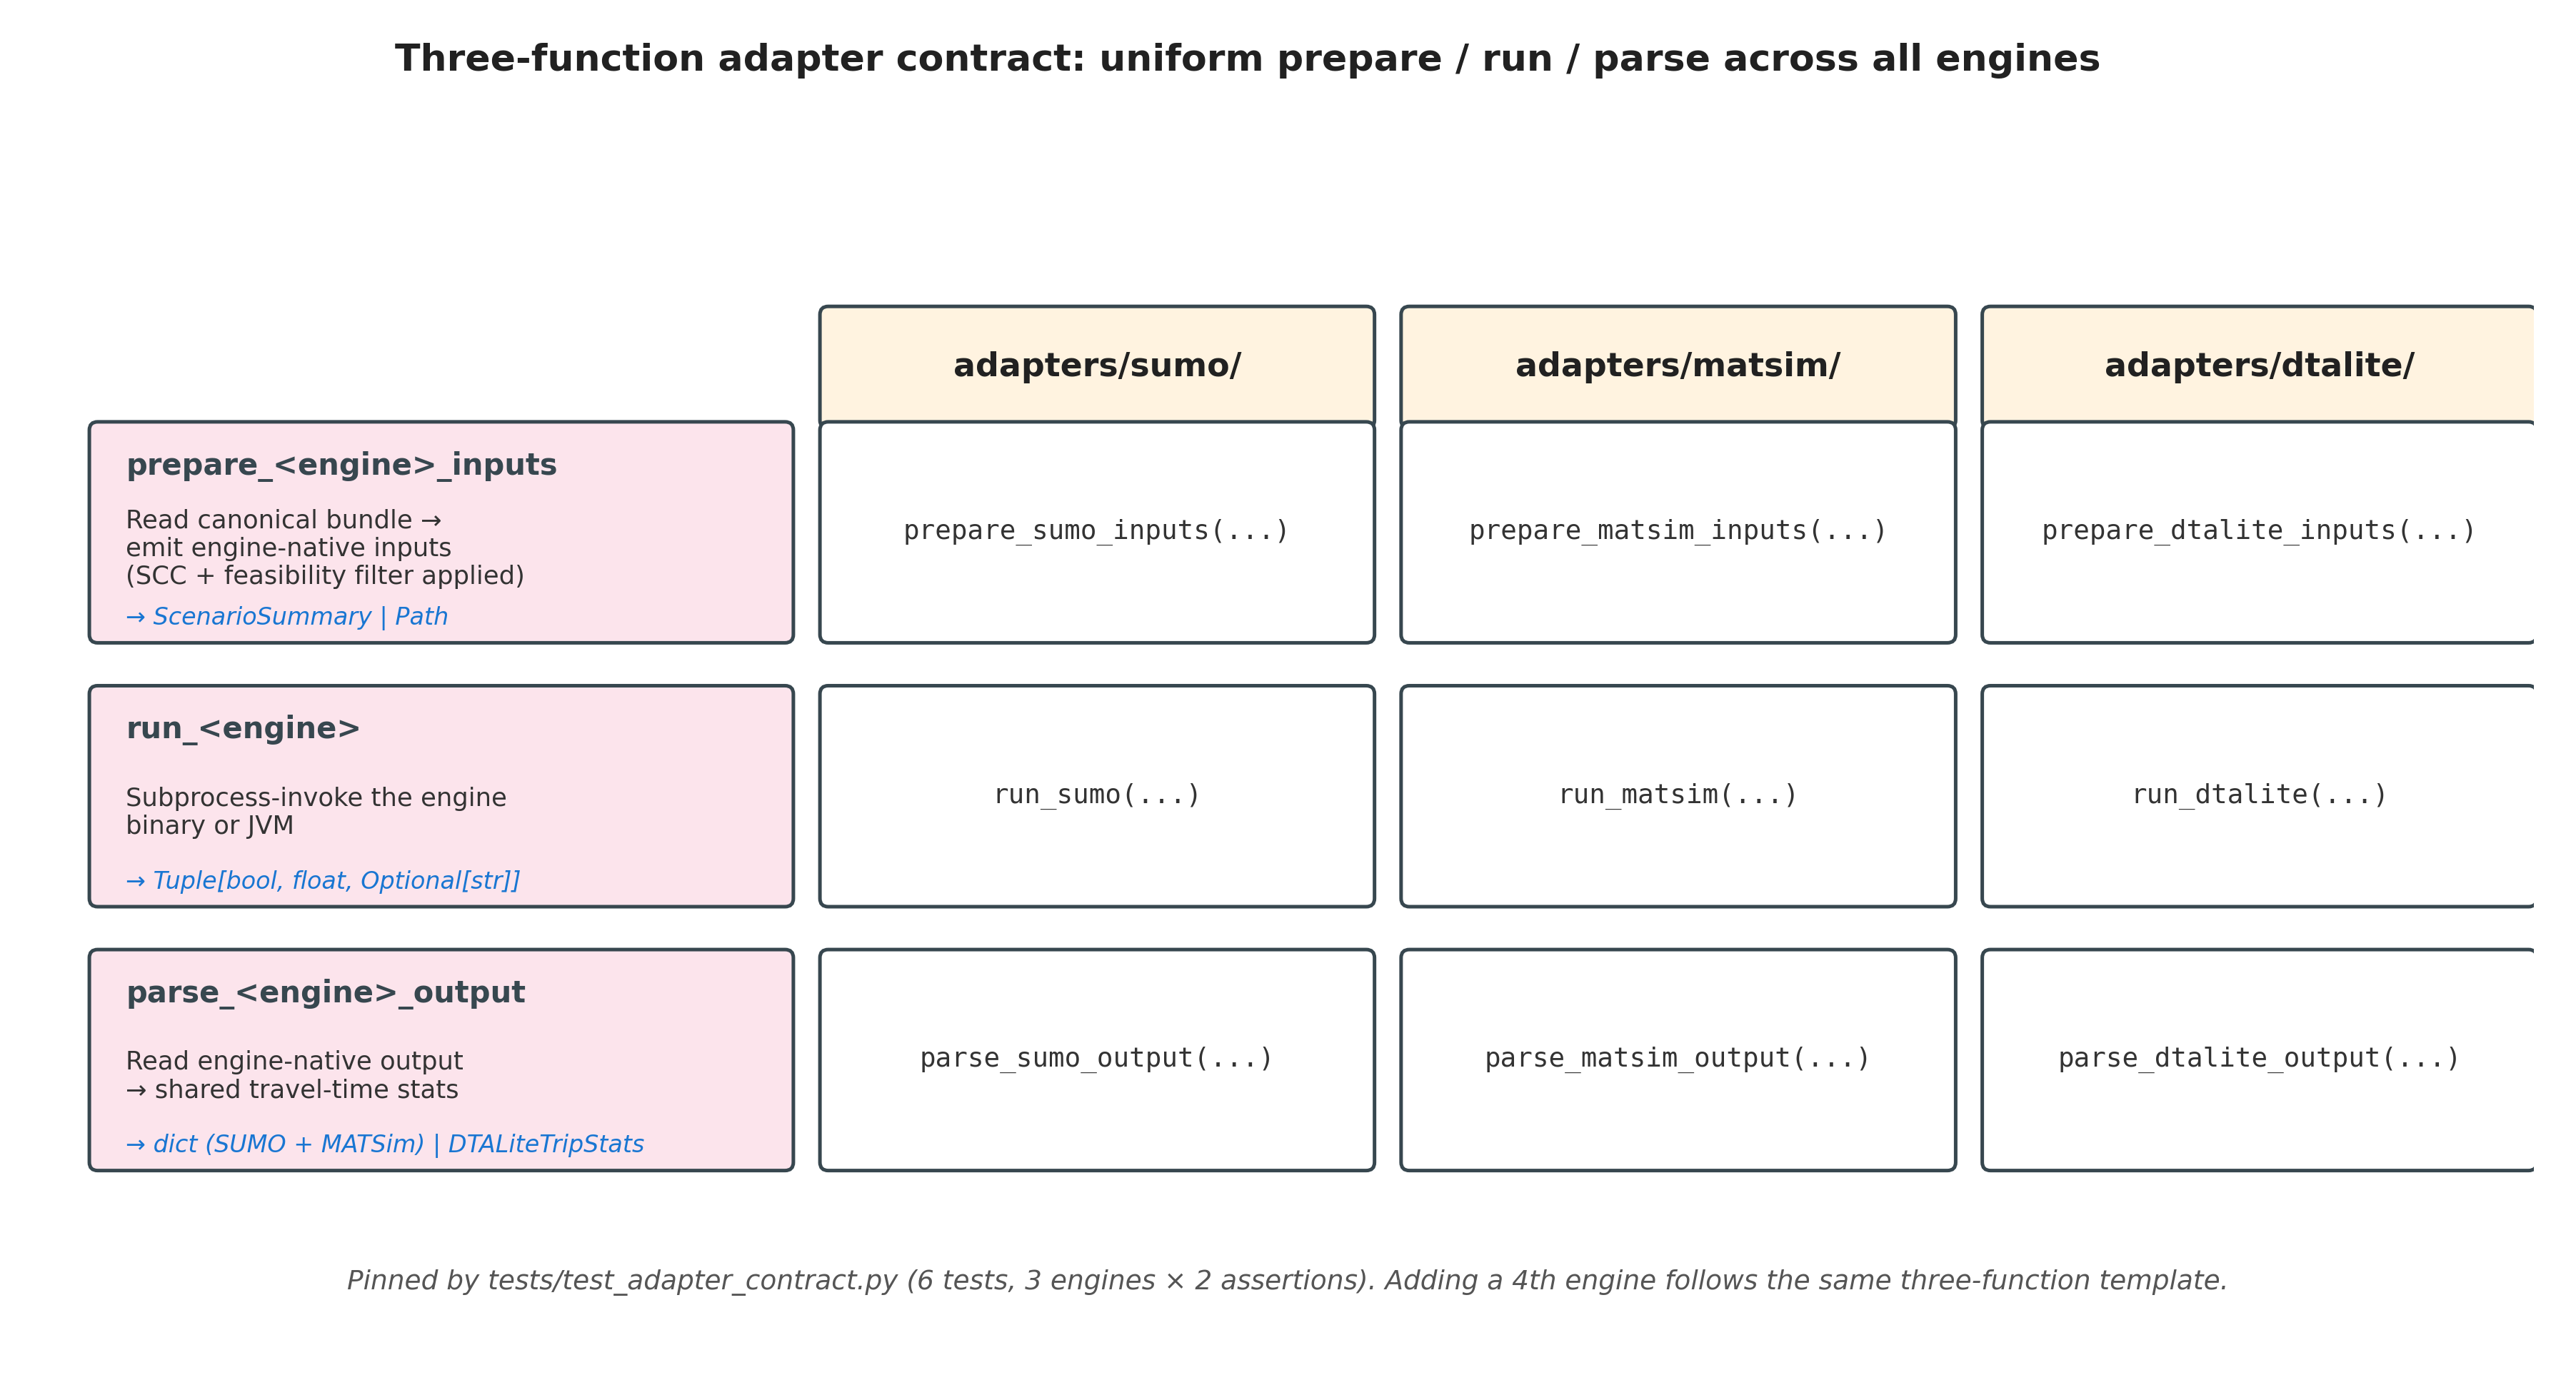
\includegraphics[keepaspectratio]{../figures/fig_3_4_adapter_contract.png}}

Figure 3.4 lays out the three-function adapter contract as a 3×3 grid:
three rows (\texttt{prepare\_\textless{}engine\textgreater{}\_inputs},
\texttt{run\_\textless{}engine\textgreater{}},
\texttt{parse\_\textless{}engine\textgreater{}\_output}) × three columns
(SUMO, MATSim, DTALite). Each cell shows the per-engine function
signature; the left labels describe the shared contract semantics and
return type. The \texttt{prepare\_} functions consume the canonical
bundle and emit engine-native inputs after applying the shared SCC +
feasibility filter and (Phase 14+) consuming canonical\_routes. The
\texttt{run\_} functions invoke the engine binary or JVM as a subprocess
and return \texttt{(success,\ runtime\_s,\ error\_msg)}. The
\texttt{parse\_} functions read engine-native outputs and return
travel-time stats --- a plain dict for SUMO + MATSim, a richer
\texttt{DTALiteTripStats} dataclass for DTALite. The contract is pinned
by \texttt{tests/test\_adapter\_contract.py} (6 tests = 3 engines × 2
assertions); adding a fourth engine follows the same template.

\subsection{Adapter Architecture}\label{341-adapter-architecture}

Each adapter implements a common operational pattern:

\begin{Shaded}
\begin{Highlighting}[]
\KeywordTok{class}\NormalTok{ SimulatorAdapter(Protocol):}
    \KeywordTok{def}\NormalTok{ prepare\_inputs(}\VariableTok{self}\NormalTok{, scenario\_path: Path, output\_dir: Path) }\OperatorTok{{-}\textgreater{}} \VariableTok{None}\NormalTok{:}
        \CommentTok{"""Convert canonical bundle to simulator{-}specific inputs."""}

    \KeywordTok{def}\NormalTok{ run\_simulation(}\VariableTok{self}\NormalTok{, config\_path: Path, }\OperatorTok{**}\NormalTok{kwargs) }\OperatorTok{{-}\textgreater{}}\NormalTok{ SimulationResult:}
        \CommentTok{"""Execute the simulator and return results."""}

    \KeywordTok{def}\NormalTok{ parse\_outputs(}\VariableTok{self}\NormalTok{, output\_dir: Path) }\OperatorTok{{-}\textgreater{}}\NormalTok{ SimulationMetrics:}
        \CommentTok{"""Extract metrics from simulator outputs."""}
\end{Highlighting}
\end{Shaded}

\textbf{Conversion guarantees:}

\begin{itemize}
\tightlist
\item
  \textbf{Deterministic}: Given the same canonical input and adapter
  version, the output is byte-identical
\item
  \textbf{Lossless (within schema)}: All canonical attributes are
  mapped; no information is dropped
\item
  \textbf{Documented}: Every mapping decision is recorded in
  \texttt{adapters/\textless{}engine\textgreater{}/MAPPING.md}
\item
  \textbf{Cross-engine vehicle alignment} (V11+): All three adapters
  source vehicle parameters from a single shared module
  \texttt{adapters/common/vehicle\_types.py}. Pre-V11 each adapter
  declared its own values inline (SUMO inherited the implicit
  \texttt{DEFAULT\_VEHTYPE}, MATSim hardcoded \texttt{length=7.5} and
  \texttt{width=1.0}), with the cross-engine equivalence undocumented
  and untested. The canonical SimForge car is now a 5.0 m sedan with a
  2.5 m gap, 1.8 m wide, 40 m/s max speed, PCE 1.0. SUMO emits
  \texttt{length="5.0"\ minGap="2.5"} (physical convention); MATSim
  emits \texttt{\textless{}length\ meter="7.5"/\textgreater{}}
  (effective-spacing convention = SUMO\textquotesingle s length +
  minGap); DTALite consumes \texttt{PCE\ =\ 1.0} (link-capacity
  convention). The equivalence is pinned by
  \texttt{tests/test\_vehicle\_types.py::TestCrossEngineEquivalence}.
  Within-bucket heterogeneity (motorcycles, taxis, freight) is post-V11
  work and remains a documented limitation.
\end{itemize}

\subsection{SUMO Adapter}\label{342-sumo-adapter}

\textbf{Simulator}: SUMO (Simulation of Urban Mobility) --- microscopic
traffic simulator modeling individual vehicles with car-following
(Krauss model) and lane-changing behavior.

\textbf{Supported modes}: Microscopic (default) and Mesoscopic
(queue-based, \textasciitilde100× faster)

\textbf{Conversion pipeline:}

\begin{verbatim}
CANONICAL                           SUMO
────────────────────────────────────────────────
network.xml  ──► nodes.nod.xml ─┐
                 edges.edg.xml ─┴─► netconvert ──► net.net.xml
demand.csv   ──► routes.rou.xml (with BFS routing)
signals.xml  ──► (embedded in net.net.xml via netconvert)
config.xml   ──► scenario.sumocfg
\end{verbatim}

\textbf{Key mapping decisions:}

\begin{longtable}[]{@{}lll@{}}
\toprule\noalign{}
Canonical & SUMO & Transformation \\
\midrule\noalign{}
\endhead
\bottomrule\noalign{}
\endlastfoot
\texttt{node\ (x,\ y)} & \texttt{node\ (x,\ y,\ type)} & x=lon, y=lat;
type defaults to \texttt{priority} \\
\texttt{link\ (from,\ to,\ length)} & \texttt{edge\ +\ lanes} & One edge
per link; numLanes, speed from canonical \\
\texttt{link.speed\_limit} & \texttt{edge.speed} & Direct copy (both in
m/s) \\
\texttt{link.lanes} & \texttt{edge.numLanes} & Direct copy \\
Trip (origin, dest) & Vehicle with route & State-aware BFS shortest path
on node graph (V5+ Phase 7) → edge sequence \\
\texttt{config.random\_seed} & \texttt{-\/-seed} CLI arg & Passed to
sumo/sumo-gui \\
\end{longtable}

\textbf{State-aware BFS routing (V5+ Phase 7)}: The SUMO adapter
computes shortest paths at conversion time (not at simulation time). For
each trip in demand.csv:

\begin{enumerate}
\def\labelenumi{\arabic{enumi}.}
\tightlist
\item
  Build the forbidden-move set from the
  \texttt{\textless{}turn\_restrictions\textgreater{}} block in
  \texttt{network.xml} via
  \texttt{pipeline/network/turn\_restrictions.build\_forbidden\_moves}.
\item
  Run state-aware BFS from \texttt{origin\_node\_id} to
  \texttt{destination\_node\_id} over \texttt{(node,\ last\_link)}
  states --- never traversing a
  \texttt{(from\_link,\ via\_node,\ to\_link)} triple in the forbidden
  set. Implemented at
  \texttt{pipeline/network/turn\_restrictions.shortest\_path\_with\_restrictions}.
\item
  Fall back to plain BFS if no restriction-respecting path exists (rare;
  SCC-feasible by construction).
\item
  Convert the node path to an edge sequence via the
  \texttt{edge\_lookup} dictionary.
\item
  Write as
  \texttt{\textless{}vehicle\ id="veh\_t0"\ depart="25200"\textgreater{}\textless{}route\ edges="l0\ l1\ l2"/\textgreater{}\textless{}/vehicle\textgreater{}}.
\end{enumerate}

The MATSim adapter uses the same state-aware BFS to pre-route every plan
and writes a
\texttt{\textless{}route\ type="links"\ start\_link="..."\ end\_link="..."\textgreater{}interior\textless{}/route\textgreater{}}
per the MATSim 15 \textbf{population\_v6} DTD (corrected from plans\_v4
in V11.2 --- plans\_v4\textquotesingle s
\texttt{\textless{}route\textgreater{}} element rejects
\texttt{type="links"} and treats text content as a node sequence;
population\_v6 supports both natively). The DTALite adapter emits a
sibling \texttt{movement.csv} with forbidden movements (capacity = 0,
penalty = 99999) but path4gmns 0.10.0 does not natively ingest it --- a
documented cross-engine asymmetry. Trips with no valid path
(disconnected OD pairs) are skipped and logged.

\textbf{Mesoscopic mode}: Activated via \texttt{-\/-mesosim} flag in
SUMO configuration. Uses queue-based link traversal instead of
car-following. Dramatically faster for large scenarios (100-1000×
speedup at 500K+ trips) with lower fidelity.

\textbf{netconvert invocation:}

\begin{Shaded}
\begin{Highlighting}[]
\ExtensionTok{netconvert} \AttributeTok{{-}{-}node{-}files}\NormalTok{ nodes.nod.xml }\DataTypeTok{\textbackslash{}}
           \AttributeTok{{-}{-}edge{-}files}\NormalTok{ edges.edg.xml }\DataTypeTok{\textbackslash{}}
           \AttributeTok{{-}{-}output{-}file}\NormalTok{ net.net.xml }\DataTypeTok{\textbackslash{}}
           \AttributeTok{{-}{-}no{-}turnarounds}
\end{Highlighting}
\end{Shaded}

\subsection{MATSim Adapter}\label{343-matsim-adapter}

\textbf{Simulator}: MATSim (Multi-Agent Transport Simulation) ---
activity-based, mesoscopic simulator modeling agents executing daily
activity plans.

\textbf{Conversion pipeline:}

\begin{verbatim}
CANONICAL                           MATSIM
────────────────────────────────────────────────
network.xml  ──► network.xml (MATSim DTD format)
demand.csv   ──► plans.xml (2-activity chains)
config.xml   ──► config.xml (MATSim config format) + vehicles.xml
\end{verbatim}

\textbf{Key mapping decisions:}

\begin{longtable}[]{@{}lll@{}}
\toprule\noalign{}
Canonical & MATSim & Notes \\
\midrule\noalign{}
\endhead
\bottomrule\noalign{}
\endlastfoot
Node (x, y) & Node with coords & Coordinates preserved as-is \\
Link & Link with freespeed, capacity &
\texttt{freespeed\ =\ speed\_limit}; capacity from lanes × 1800 \\
Trip (OD, time) & Person with 2-activity plan & home(origin) →
work(destination) \\
Mode & Leg mode & car/transit/bike mapped to MATSim modes \\
Random seed & \texttt{config/global/randomSeed} & Propagated to MATSim
config XML \\
\end{longtable}

\textbf{Demand conversion}: Each canonical trip becomes a MATSim agent
with a 2-activity plan:

\begin{Shaded}
\begin{Highlighting}[]
\NormalTok{\textless{}}\KeywordTok{person}\OtherTok{ id=}\StringTok{"person\_t0"}\NormalTok{\textgreater{}}
\NormalTok{  \textless{}}\KeywordTok{plan}\OtherTok{ selected=}\StringTok{"yes"}\NormalTok{\textgreater{}}
\NormalTok{    \textless{}}\KeywordTok{activity}\OtherTok{ type=}\StringTok{"home"}\OtherTok{ link=}\StringTok{"l\_near\_origin"}\OtherTok{ end\_time=}\StringTok{"07:00:00"}\NormalTok{/\textgreater{}}
\NormalTok{    \textless{}}\KeywordTok{leg}\OtherTok{ mode=}\StringTok{"car"}\NormalTok{/\textgreater{}}
\NormalTok{    \textless{}}\KeywordTok{activity}\OtherTok{ type=}\StringTok{"work"}\OtherTok{ link=}\StringTok{"l\_near\_destination"}\NormalTok{/\textgreater{}}
\NormalTok{  \textless{}/}\KeywordTok{plan}\NormalTok{\textgreater{}}
\NormalTok{\textless{}/}\KeywordTok{person}\NormalTok{\textgreater{}}
\end{Highlighting}
\end{Shaded}

\textbf{Single-iteration mode}: For fair comparison with SUMO, MATSim is
configured with \texttt{lastIteration=0}, disabling the iterative
replanning loop that MATSim normally uses to reach user equilibrium.

\textbf{Java/JAR detection}: The adapter auto-detects the Java runtime
and MATSim JAR location:

\begin{enumerate}
\def\labelenumi{\arabic{enumi}.}
\tightlist
\item
  Checks \texttt{JAVA\_HOME}, then \texttt{PATH}, then common install
  locations
\item
  Locates \texttt{matsim-15.0.jar} in the \texttt{lib/} directory
\item
  Constructs classpath including all dependency JARs
\end{enumerate}

\begin{longtable}[]{@{}lll@{}}
\toprule\noalign{}
Aspect & SUMO & MATSim \\
\midrule\noalign{}
\endhead
\bottomrule\noalign{}
\endlastfoot
Resolution & Vehicle-level & Agent-level \\
Demand representation & OD routes & Activity plans \\
Traffic flow & Car-following & Queue-based (mesoscopic) \\
Typical iterations & 1 & 1 (forced for fair comparison) \\
Startup overhead & \textasciitilde0.1s & \textasciitilde5-7s (JVM
warmup) \\
\end{longtable}

\subsection{DTALite Adapter}\label{344-dtalite-adapter}

\textbf{Simulator}: DTALite --- CPU-only mesoscopic Dynamic Traffic
Assignment engine distributed under Apache 2.0 license, bundled inside
the \href{https://github.com/jdlph/Path4GMNS}{\texttt{path4gmns}} Python
package. Replaces LPSim in the third-engine slot in \textbf{Version\_5}
after the LPSim integration was abandoned (see
\href{../engines/LPSIM_RETROSPECTIVE.md}{\texttt{doc/engines/LPSIM\_RETROSPECTIVE.md}}).
The selection rationale and the two ruled-out alternatives (CityFlow,
POLARIS) are documented in
\href{../engines/THIRD_ENGINE_OPTIONS.md}{\texttt{doc/engines/THIRD\_ENGINE\_OPTIONS.md}}.

\textbf{Conversion} (Canonical → GMNS schema):

\begin{longtable}[]{@{}lll@{}}
\toprule\noalign{}
File & Canonical & DTALite (GMNS) \\
\midrule\noalign{}
\endhead
\bottomrule\noalign{}
\endlastfoot
Nodes & \texttt{network.xml}
\texttt{\textless{}node\ id="n123"\ x="…"\ y="…"/\textgreater{}} &
\texttt{node.csv} columns
\texttt{node\_id,\ zone\_id,\ x\_coord,\ y\_coord,\ production,\ attraction} \\
Edges & \texttt{network.xml}
\texttt{\textless{}link\ id="l456"\ from="n10"\ to="n11"\ length="120.5"\ speed\_limit="13.9"\ lanes="2"/\textgreater{}}
& \texttt{link.csv} columns
\texttt{link\_id,\ from\_node\_id,\ to\_node\_id,\ length\ (km),\ lanes,\ free\_speed\ (km/h),\ capacity,\ link\_type,\ VDF\_fftt1,\ VDF\_alpha1,\ VDF\_beta1}
(m → km, m/s × 3.6 → km/h) \\
Demand & \texttt{demand.csv}
\texttt{trip\_id,\ origin\_node\_id,\ destination\_node\_id,\ departure\_time\_s,\ mode}
& \texttt{demand.csv} columns
\texttt{o\_zone\_id,\ d\_zone\_id,\ volume} (trips aggregated by OD
pair) \\
Config & \texttt{config.xml}
\texttt{\textless{}time\ start\_time\_s="25200"\ end\_time\_s="28800"/\textgreater{}}
& \texttt{settings.csv} (\texttt{{[}demand\_period{]}} AM 0700\_0800) +
\texttt{settings.yml} mirror for the path4gmns Python wrapper \\
\end{longtable}

\textbf{Demand-driven zoning}: DTALite\textquotesingle s UE assignment
iterates over zones, running label-correcting shortest-path from each
zone in every outer iteration. Treating every node as a zone (the naive
approach) produced 20,058-zone runs that took minutes per outer
iteration on chicago\_1k\_car. The adapter therefore promotes only nodes
that appear as origin or destination in the demand to GMNS zones
(\textasciitilde1,800 zones for chicago\_1k\_car); transit-only
intersections retain network connectivity but are skipped in the UE
loop. Runtime drops from "minutes" to \textasciitilde5 seconds at the
bundled scenario size.

\textbf{Fidelity trade-off --- departure timing}:
DTALite\textquotesingle s GMNS demand format does not include a per-trip
departure column; trips are aggregated by (origin, destination) into a
count \texttt{volume}. Departures are distributed uniformly inside the
\texttt{{[}demand\_period{]}} window (default 0700-0800 --- controlled
by \texttt{DTALiteConfig}). The canonical \texttt{departure\_time\_s}
precision available to SUMO and MATSim is therefore not exposed to
DTALite. This is the single cleanest difference between the three
engines from a demand-modeling perspective and is documented in
\texttt{adapters/dtalite/MAPPING.md} for full audit trail.

\textbf{Determinism}: DTALite is fully deterministic. The UE algorithm
(Method of Successive Averages / Frank-Wolfe) iterates in fixed order
with no atomic reductions and no GPU non-determinism. R-score is
expected to be 1.0 across N=5 repeats with the same inputs, matching
SUMO mesoscopic and MATSim with \texttt{lastIteration=0}. (This
determinism is one of the technical reasons DTALite was preferred over
LPSim, whose \texttt{atomicAdd} GPU reductions would have forced an
explanatory footnote on every reproducibility number --- see
\texttt{LPSIM\_RETROSPECTIVE.md} §5.)

\textbf{Binary discovery}: \texttt{is\_dtalite\_available()} checks both
that \texttt{path4gmns} is importable AND that the platform-specific
bundled binary (\texttt{DTALiteMM\_arm.dylib} /
\texttt{DTALiteMM\_x86.dylib} / \texttt{DTALiteMM.so} /
\texttt{DTALiteMM.dll}) exists in the package\textquotesingle s
\texttt{bin/} directory. With path4gmns not installed,
\texttt{run\_dtalite()} returns a clean \texttt{RunResult} failure with
the install command (\texttt{uv\ pip\ install\ path4gmns}) --- no silent
fallback (the failure mode that motivated dropping QarSUMO).

\textbf{Implementation note} --- DTALiteClassic vs DTALiteMultimodal:
path4gmns 0.10.0 ships two DTALite binaries. The adapter calls
\texttt{DTALiteClassic} (mode 1 = path-based UE), not the newer
\texttt{DTALiteMultimodal} wrapper. The multimodal binary has a
regression demanding a \texttt{mode\_type.csv} schema upstream has not
published --- even path4gmns\textquotesingle s own bundled samples fail
with
\texttt{{[}ERROR{]}\ File\ mode\_type\ does\ not\ have\ information}
when invoked fresh. Full implementation note in
\texttt{adapters/dtalite/MAPPING.md}.

\textbf{Performance expectation}: at SimForge scenario sizes (1k--500k
trips, ≤500k nodes) DTALite is comparable to MATSim in wallclock ---
slower than SUMO meso, faster than SUMO micro at scale. The thesis claim
is paradigm spread (microscopic + queue-based agent + DTA equilibrium),
not raw speedup; see \texttt{doc/engines/ENGINE\_COMPARISON.md} §3 for
the per-tier wallclock estimates.

\subsection{Adapter Determinism}\label{345-adapter-determinism}

All adapters enforce deterministic output through:

\begin{enumerate}
\def\labelenumi{\arabic{enumi}.}
\tightlist
\item
  \textbf{Sorted iteration}: All XML elements emitted in sorted order
  (by node ID, link ID, etc.) --- avoids hash-set iteration order
  differences
\item
  \textbf{Fixed random seeds}: The canonical \texttt{random\_seed} from
  config.xml is propagated to all simulator-level random seed parameters
\item
  \textbf{Version pinning}: Adapter code is versioned alongside the
  framework; simulator versions are recorded in metadata
\item
  \textbf{Hash verification}: Post-conversion, the adapter can
  re-validate that canonical inputs haven\textquotesingle t drifted
  since scenario generation
\end{enumerate}

\begin{center}\rule{0.5\linewidth}{0.5pt}\end{center}

\section{Execution Harness}\label{35-execution-harness}

\subsection{Run Specification
Schema}\label{351-run-specification-schema}

Benchmark runs are defined via YAML runspec files that specify the
experimental matrix:

\begin{Shaded}
\begin{Highlighting}[]
\FunctionTok{name}\KeywordTok{:}\AttributeTok{ stress\_test}
\FunctionTok{description}\KeywordTok{:}\AttributeTok{ End{-}to{-}end stress test across all engines and modes.}
\FunctionTok{output\_dir}\KeywordTok{:}\AttributeTok{ runs/benchmark\_small}

\FunctionTok{runs}\KeywordTok{:}
\AttributeTok{  }\KeywordTok{{-}}\AttributeTok{ }\FunctionTok{scenario\_id}\KeywordTok{:}\AttributeTok{ chicago\_1k\_car}
\AttributeTok{    }\FunctionTok{scenario\_path}\KeywordTok{:}\AttributeTok{ scenarios/chicago\_1k\_car}
\AttributeTok{    }\FunctionTok{engine}\KeywordTok{:}\AttributeTok{ sumo}
\AttributeTok{    }\FunctionTok{mode}\KeywordTok{:}\AttributeTok{ mesoscopic}
\AttributeTok{    }\FunctionTok{repeats}\KeywordTok{:}\AttributeTok{ }\DecValTok{3}
\AttributeTok{    }\FunctionTok{seed}\KeywordTok{:}\AttributeTok{ }\DecValTok{42}
\AttributeTok{    }\FunctionTok{timeout\_s}\KeywordTok{:}\AttributeTok{ }\DecValTok{300}

\AttributeTok{  }\KeywordTok{{-}}\AttributeTok{ }\FunctionTok{scenario\_id}\KeywordTok{:}\AttributeTok{ chicago\_1k\_car}
\AttributeTok{    }\FunctionTok{scenario\_path}\KeywordTok{:}\AttributeTok{ scenarios/chicago\_1k\_car}
\AttributeTok{    }\FunctionTok{engine}\KeywordTok{:}\AttributeTok{ matsim}
\AttributeTok{    }\FunctionTok{mode}\KeywordTok{:}\AttributeTok{ mesoscopic}
\AttributeTok{    }\FunctionTok{repeats}\KeywordTok{:}\AttributeTok{ }\DecValTok{2}
\AttributeTok{    }\FunctionTok{seed}\KeywordTok{:}\AttributeTok{ }\DecValTok{42}
\AttributeTok{    }\FunctionTok{timeout\_s}\KeywordTok{:}\AttributeTok{ }\DecValTok{600}
\end{Highlighting}
\end{Shaded}

\textbf{RunConfig fields:}

\begin{longtable}[]{@{}lll@{}}
\toprule\noalign{}
Field & Type & Description \\
\midrule\noalign{}
\endhead
\bottomrule\noalign{}
\endlastfoot
\texttt{scenario\_id} & string & Human-readable scenario identifier \\
\texttt{scenario\_path} & string & Path to canonical scenario bundle \\
\texttt{engine} & string & Simulator: \texttt{sumo}, \texttt{matsim},
\texttt{dtalite} \\
\texttt{mode} & enum & \texttt{microscopic} or \texttt{mesoscopic} \\
\texttt{repeats} & int & Number of repeated runs (for reproducibility
analysis) \\
\texttt{seed} & int & Base seed (incremented per repeat: 42, 43, 44) \\
\texttt{timeout\_s} & int & Maximum wall-clock time per run \\
\end{longtable}

\textbf{SimulationMode enum:}

\begin{Shaded}
\begin{Highlighting}[]
\KeywordTok{class}\NormalTok{ SimulationMode(}\BuiltInTok{str}\NormalTok{, Enum):}
\NormalTok{    MICROSCOPIC }\OperatorTok{=} \StringTok{"microscopic"}  \CommentTok{\# Car{-}following + lane{-}changing (accurate, slow)}
\NormalTok{    MESOSCOPIC }\OperatorTok{=} \StringTok{"mesoscopic"}    \CommentTok{\# Queue{-}based edge traversal (fast, \textasciitilde{}100× speedup)}
\end{Highlighting}
\end{Shaded}

\subsection{Benchmark Execution
Pipeline}\label{352-benchmark-execution-pipeline}

The \texttt{BenchmarkHarness} orchestrates the full execution lifecycle:

\begin{verbatim}
For each (scenario, engine, mode, seed):
    1. Validate canonical bundle  ──► abort if invalid
    2. Prepare simulator inputs   ──► adapter.prepare_inputs()
    3. Execute simulation         ──► adapter.run_simulation()
    4. Collect raw outputs        ──► tripinfo.xml, summary.xml, etc.
    5. Compute metrics            ──► adapter.parse_outputs()
    6. Record RunResult           ──► JSON serializable
\end{verbatim}

\textbf{Progress tracking}: The \texttt{StickyProgress} bar displays
real-time progress with completion ratio, ✓/✗ counts, elapsed clock, and
a Braille spinner heartbeat (V11.2+ removed the ETA estimate ---
SimForge cells are heterogeneous, so a running-mean ETA swings between
unhelpful extremes):

\begin{verbatim}
[████████████████████░░░░░░░░░░░░░░░░░░░░] 52.3%  ⠼  47/90 runs  ✓45 ✗2  elapsed 12m 30s
\end{verbatim}

\textbf{Output structure:}

\begin{verbatim}
runs/
└── benchmark_20250615_143022/
    ├── chicago_1k_car_sumo_meso_seed42/
    │   ├── net.net.xml
    │   ├── routes.rou.xml
    │   ├── scenario.sumocfg
    │   └── output/
    │       ├── tripinfo.xml
    │       └── summary.xml
    ├── chicago_1k_car_matsim_meso_seed42/
    │   ├── network.xml
    │   ├── plans.xml
    │   ├── config.xml
    │   └── output/
    │       └── output_events.xml.gz
    └── benchmark_results_<runspec>.json
\end{verbatim}

\subsection{Result Aggregation}\label{353-result-aggregation}

All run results are serialized to
\texttt{benchmark\_results\_\textless{}runspec\textgreater{}.json}:

\begin{Shaded}
\begin{Highlighting}[]
\FunctionTok{\{}
  \DataTypeTok{"runspec\_name"}\FunctionTok{:} \StringTok{"stress\_test"}\FunctionTok{,}
  \DataTypeTok{"started\_at"}\FunctionTok{:} \StringTok{"2026{-}04{-}19T02:05:28+00:00"}\FunctionTok{,}
  \DataTypeTok{"completed\_at"}\FunctionTok{:} \StringTok{"2026{-}04{-}19T02:06:19+00:00"}\FunctionTok{,}
  \DataTypeTok{"total\_runs"}\FunctionTok{:} \DecValTok{22}\FunctionTok{,}
  \DataTypeTok{"successful\_runs"}\FunctionTok{:} \DecValTok{22}\FunctionTok{,}
  \DataTypeTok{"failed\_runs"}\FunctionTok{:} \DecValTok{0}\FunctionTok{,}
  \DataTypeTok{"results"}\FunctionTok{:} \OtherTok{[}
    \FunctionTok{\{}
      \DataTypeTok{"scenario"}\FunctionTok{:} \StringTok{"chicago\_1k\_car"}\FunctionTok{,}
      \DataTypeTok{"engine"}\FunctionTok{:} \StringTok{"sumo"}\FunctionTok{,}
      \DataTypeTok{"mode"}\FunctionTok{:} \StringTok{"meso"}\FunctionTok{,}
      \DataTypeTok{"seed"}\FunctionTok{:} \DecValTok{42}\FunctionTok{,}
      \DataTypeTok{"status"}\FunctionTok{:} \StringTok{"success"}\FunctionTok{,}
      \DataTypeTok{"runtime\_s"}\FunctionTok{:} \FloatTok{0.279}\FunctionTok{,}
      \DataTypeTok{"metrics"}\FunctionTok{:} \FunctionTok{\{}
        \DataTypeTok{"travel\_time"}\FunctionTok{:} \FunctionTok{\{}
          \DataTypeTok{"mean"}\FunctionTok{:} \FloatTok{204.18}\FunctionTok{,}
          \DataTypeTok{"p95"}\FunctionTok{:} \FloatTok{406.0}\FunctionTok{,}
          \DataTypeTok{"trip\_count"}\FunctionTok{:} \DecValTok{996}
        \FunctionTok{\}}
      \FunctionTok{\}}
    \FunctionTok{\}}
  \OtherTok{]}
\FunctionTok{\}}
\end{Highlighting}
\end{Shaded}

\begin{center}\rule{0.5\linewidth}{0.5pt}\end{center}

\section{Evaluation Metrics}\label{36-evaluation-metrics}

\pandocbounded{
\includegraphics[keepaspectratio]{../figures/fig_3_6_fairness_audit_flow.png}}

Figure 3.6 walks through the cross-engine fairness audit
(\texttt{evaluation/audit\_fairness.py}) as a vertical flow. Input is a
run directory containing per-engine cells. The audit then runs five
questions in order, each producing a verdict line in the audit output:
\textbf{Q1} (mandatory) --- byte-identical feasibility verdicts across
all engines; \textbf{Q2} (mandatory) --- byte-identical SCC node + link
counts; \textbf{Q3} (mandatory) --- every engine simulated the same
trip-count target; \textbf{Q4} (informational) --- cross-engine mean-TT
comparison (the paradigm-divergence signal that drives §5.6.2);
\textbf{Q5} (informational) --- V5+ demand-composition tally. Q1-Q3 are
the \emph{fairness contract} --- they must PASS for the cross-engine
comparison to be attributable to engine paradigm rather than input
asymmetry. Q4 + Q5 are the interpretive readouts that make the
fairness-contract guarantee actionable for the chapter-5
paradigm-divergence narrative.

\subsection{Metric Categories}\label{361-metric-categories}

The evaluation framework measures three orthogonal quality dimensions:

\begin{longtable}[]{@{}lll@{}}
\toprule\noalign{}
Dimension & Question & Metrics \\
\midrule\noalign{}
\endhead
\bottomrule\noalign{}
\endlastfoot
\textbf{Fidelity} & How closely do simulators agree with each other? &
RMSE, GEH, KS statistic \\
\textbf{Scalability} & How efficiently does each simulator use compute
resources? & Runtime, throughput, SRT \\
\textbf{Reproducibility} & How consistent are results across repeated
runs? & Reproducibility index \(R\) \\
\end{longtable}

\subsection{Fidelity Metrics}\label{362-fidelity-metrics}

\textbf{Root Mean Square Error (RMSE):}

\[\text{RMSE} = \sqrt{\frac{1}{n}\sum_{i=1}^{n}(y_i - \hat{y}_i)^2}\]

Applied to link-level traffic counts or travel times across two
simulators. Lower RMSE indicates closer agreement. Units match the input
(seconds for travel time, vehicles for counts).

\textbf{GEH Statistic} (Geoffrey E. Havers):

\[\text{GEH} = \sqrt{\frac{2(M - C)^2}{M + C}}\]

where \(M\) is the modeled value and \(C\) is the comparison/observed
value. Standard in traffic engineering (UK DfT, FHWA):

\begin{longtable}[]{@{}lll@{}}
\toprule\noalign{}
GEH Range & Interpretation & Action \\
\midrule\noalign{}
\endhead
\bottomrule\noalign{}
\endlastfoot
\textless{} 5 & Acceptable fit & No action needed \\
5 -- 10 & Warrants investigation & Check individual links \\
\textgreater{} 10 & Poor fit & Model needs revision \\
\end{longtable}

The implementation computes per-link GEH and reports both the
\textbf{mean GEH} and the \textbf{percentage of links with GEH
\textless{} 5} (the industry-standard acceptance criterion).

\textbf{Kolmogorov-Smirnov Statistic:}

\[D = \sup_x |F_1(x) - F_2(x)|\]

Compares the empirical cumulative distribution functions (CDFs) of
travel time distributions from two simulators. Critical value at
significance level \(\alpha = 0.05\):

\[D_{\text{crit}} = 1.36 \sqrt{\frac{n_1 + n_2}{n_1 \cdot n_2}}\]

If \(D > D_{\text{crit}}\), the distributions are statistically
different at the 5\% level.

\subsection{Scalability Metrics}\label{363-scalability-metrics}

\textbf{Wall-clock runtime}: Measured via \texttt{time.perf\_counter()}
context manager for nanosecond precision:

\begin{Shaded}
\begin{Highlighting}[]
\KeywordTok{class}\NormalTok{ SimulationTimer:}
    \KeywordTok{def} \FunctionTok{\_\_enter\_\_}\NormalTok{(}\VariableTok{self}\NormalTok{):}
        \VariableTok{self}\NormalTok{.start\_time }\OperatorTok{=}\NormalTok{ time.perf\_counter()}
        \ControlFlowTok{return} \VariableTok{self}
    \KeywordTok{def} \FunctionTok{\_\_exit\_\_}\NormalTok{(}\VariableTok{self}\NormalTok{, }\OperatorTok{*}\NormalTok{args):}
        \VariableTok{self}\NormalTok{.elapsed\_seconds }\OperatorTok{=}\NormalTok{ time.perf\_counter() }\OperatorTok{{-}} \VariableTok{self}\NormalTok{.start\_time}
\end{Highlighting}
\end{Shaded}

\textbf{Throughput:}

\[\text{Throughput} = \frac{\text{vehicles completed}}{\text{wall-clock seconds}}\]

Units: vehicles/second. Higher is better. Enables direct comparison
across hardware.

\textbf{Simulated-to-Real-Time ratio (SRT):}

\[\text{SRT} = \frac{T_\text{simulated}}{T_\text{wall-clock}}\]

SRT \textgreater{} 1 means the simulator is faster than real time. SRT =
10 means 1 hour of traffic simulated in 6 minutes.

\textbf{Normalized throughput} (when hardware info available):

\[\text{Throughput}_\text{core} = \frac{\text{Throughput}}{\text{CPU cores}}\]

\[\text{Throughput}_\text{watt} = \frac{\text{Throughput}}{\text{TDP (watts)}}\]

\textbf{Hardware detection}: The framework auto-detects CPU model, core
count, and memory via platform APIs.

\subsection{Reproducibility
Metric}\label{364-reproducibility-metric}

\textbf{Coefficient of Reproducibility:}

\[R = 1 - \frac{\sigma}{\mu}\]

where \(\sigma\) is standard deviation and \(\mu\) is mean of a KPI
across repeated runs with different random seeds.

\begin{longtable}[]{@{}ll@{}}
\toprule\noalign{}
\(R\) Range & Interpretation \\
\midrule\noalign{}
\endhead
\bottomrule\noalign{}
\endlastfoot
\(R \geq 0.99\) & Excellent (near-deterministic) \\
\(0.95 \leq R < 0.99\) & Very good \\
\(0.90 \leq R < 0.95\) & Good \\
\(0.80 \leq R < 0.90\) & Acceptable \\
\(0.50 \leq R < 0.80\) & Marginal \\
\(R < 0.50\) & Poor \\
\end{longtable}

\textbf{Multi-KPI analysis}: The \texttt{MultiKPIReproducibility} class
computes \(R\) across multiple KPIs (mean travel time, p95 travel time,
throughput, etc.) and reports the \textbf{overall reproducibility} as
the average \(R\) across all KPIs.

\textbf{Edge case handling:}

\begin{itemize}
\tightlist
\item
  All values identical → \(R = 1.0\) (perfect reproducibility)
\item
  Mean near zero → special handling to avoid division instability
\item
  Fewer than 2 runs → error (meaningless without repetition)
\end{itemize}

\subsection{Travel Time
Extraction}\label{365-travel-time-extraction}

The \texttt{travel\_time} module parses simulator-specific output files
to extract trip-level metrics:

\textbf{SUMO tripinfo.xml parsing:}

\begin{Shaded}
\begin{Highlighting}[]
\NormalTok{\textless{}}\KeywordTok{tripinfo}\OtherTok{ id=}\StringTok{"veh\_t0"}\OtherTok{ depart=}\StringTok{"25200.00"}\OtherTok{ departDelay=}\StringTok{"0.00"}
\OtherTok{          arrival=}\StringTok{"25445.30"}\OtherTok{ duration=}\StringTok{"245.30"}\OtherTok{ routeLength=}\StringTok{"3240.1"}\NormalTok{/\textgreater{}}
\end{Highlighting}
\end{Shaded}

Extracted fields: \texttt{duration} (travel time in seconds) for each
completed trip.

\textbf{Computed statistics:}

\begin{longtable}[]{@{}ll@{}}
\toprule\noalign{}
Statistic & Formula \\
\midrule\noalign{}
\endhead
\bottomrule\noalign{}
\endlastfoot
Mean travel time & \(\bar{t} = \frac{1}{n}\sum_i t_i\) \\
P95 travel time & 95th percentile of sorted durations \\
Trip completion count & Number of trips with arrival time \textless{}
end\_time \\
\end{longtable}

\begin{center}\rule{0.5\linewidth}{0.5pt}\end{center}

\section{Implementation Quality}\label{37-implementation-quality}

\subsection{Test Suite}\label{371-test-suite}

The framework includes \textbf{\textasciitilde639 tests} with all 5
bundles generated (\texttt{chicago\_1k\_car}, \texttt{nyc\_10k\_car},
\texttt{la\_50k\_car}, \texttt{chicago\_200k\_car},
\texttt{nyc\_500k\_car}). The base count is roughly 450 tests plus 36
parametrized integrity tests per bundle in \texttt{scenarios/}. Phase 14
additions (\texttt{test\_canonical\_routes.py} byte-identity guards) and
Phase 14.13 additions (\texttt{test\_run\_benchmark.py} cache-hoist
guards) account for most of the count growth over the pre-Phase-14
baseline of \textasciitilde574 tests.

\begin{longtable}[]{@{}lll@{}}
\toprule\noalign{}
Test Module & Tests & What It Validates \\
\midrule\noalign{}
\endhead
\bottomrule\noalign{}
\endlastfoot
\texttt{test\_adapter\_determinism.py} & 8 & Byte-identical outputs from
identical inputs \\
\texttt{test\_sumo\_adapter.py} & 4 & SUMO conversion: network, routes,
config \\
\texttt{test\_matsim\_adapter.py} & 26 & MATSim adapter (incl. Phase
12.1 route-text format pin) \\
\texttt{test\_fidelity\_metrics.py} & 21 & RMSE, GEH, KS computation
correctness \\
\texttt{test\_metrics\_travel\_time.py} & 2 & SUMO tripinfo parsing \\
\texttt{test\_reproducibility\_metrics.py} & 15 & R-index computation,
edge cases, interpretation \\
\texttt{test\_scalability\_metrics.py} & 8 & Timer, throughput, hardware
detection \\
\texttt{test\_validator.py} & 2 & Bundle validation: valid and invalid
bundles \\
\texttt{test\_scenario\_data\_integrity.py} & 36 × N & 7 classes × 36
tests/scenario × N bundles in \texttt{scenarios/} (108 for 3 tracked,
180 for all 5) \\
\texttt{test\_pipeline\_e2e.py} & 20 & Bad data detection, routing,
adapter robustness \\
\texttt{test\_scc.py} & 14 & Iterative Kosaraju + parsing \\
\texttt{test\_feasibility.py} & 19 & Shared cross-engine trip filter +
V5 mode-aware feasibility \\
\texttt{test\_analyze\_benchmark.py} & 24 & Mode-aware grouping + Phase
10 demand composition table \\
\texttt{test\_audit\_fairness.py} & 40 & Q1--Q5 audit helpers + 5-layout
detector (Phase 12+ mode-segmented + back-compat fallbacks) \\
\texttt{test\_run\_benchmark.py} (Phase 12+) & 12 & BenchmarkHarness
explicit-output, prep-cache, bundle-hash invalidation, scoped\_base
collapse (Phase 12.2) \\
\texttt{test\_confidence.py} & 18 & Student\textquotesingle s-t 95 \% CI
core + edge cases \\
\texttt{test\_osm\_fetch.py} & 20 & OSM/Overpass fetch (mocked), bbox
validation, cache pin \\
\texttt{test\_demand\_generators.py} & 21 & Uniform/gravity/peak-hour
generators, SCC restriction \\
\texttt{test\_demand\_composition.py} (V5+ Phase 10) & 7 &
\texttt{purpose} column tally, AM/PM peak split, pre-V5 graceful
no-op \\
\texttt{test\_parse\_model\_file.py} & 27 & ModelGen parser + V5 Phase 5
JWTRNS mapping + Phase 9 HBSchool helpers \\
\texttt{test\_turn\_restrictions.py} (V5+ Phase 7) & 17 & OSM
restriction parser, forbidden-move builder, state-aware BFS, DTALite
movement.csv \\
\texttt{test\_vehicle\_types.py} (V5+ Phase 11) & 19 & Canonical car
constants, SUMO/MATSim XML emission, cross-engine equivalence \\
\texttt{test\_dtalite\_adapter.py} & 46 & DTALite adapter: writers,
settings, demand-driven zoning, determinism, output parsing, end-to-end
smoke \\
\texttt{test\_engine\_smoke.py} & 4 & Real-binary smoke on
SUMO/MATSim/DTALite \\
\texttt{test\_adapter\_contract.py} (audit) & 6 & Three-function adapter
contract regression guard (prepare/run/parse across
SUMO+MATSim+DTALite) \\
\end{longtable}

\textbf{All \textasciitilde639 tests passing} with all 5 bundles
generated, as of the Phase 14.13 cache-hoist landing (commit
\texttt{db8d786}, 2026-05-19). Marker registry in
\texttt{pyproject.toml}; shared fixtures in \texttt{tests/conftest.py}.
Line coverage sits at \textbf{76 \%} across the adapter, pipeline, and
evaluation packages; the local gate enforces ≥70 \% via
\texttt{pytest\ -\/-cov\ -\/-cov-fail-under=70}.

\subsection{Determinism
Guarantees}\label{372-determinism-guarantees}

\begin{longtable}[]{@{}ll@{}}
\toprule\noalign{}
Mechanism & What It Ensures \\
\midrule\noalign{}
\endhead
\bottomrule\noalign{}
\endlastfoot
Fixed random seeds & All stochastic processes seeded via config.xml
\texttt{random\_seed} \\
Sorted outputs & All XML/CSV files use sorted iteration over
sets/dicts \\
SHA-256 hashes & Manifest checksums detect any input drift \\
Version pinning & \texttt{requirements.txt} specifies exact package
versions \\
Per-bundle toolchain capture &
\texttt{generation\_metadata.json::toolchain} records the Python and dep
versions that built each bundle \\
Deterministic BFS & Adapter routing uses sorted adjacency lists for
tie-breaking \\
Schedule-first hybrid (demand) & PUMS-derived workplace destinations are
deterministic per (modelgen, network, seed) triple \\
\end{longtable}

\textbf{Cross-platform reproducibility (verified).} Generation produces
byte-identical \texttt{demand.csv} and \texttt{signals.xml} across
(Apple Silicon ARM64, macOS, Python 3.13.2, osmnx 2.0.7) and (x86\_64,
RHEL Pitzer, Python 3.12.4, osmnx 2.1.0), verified empirically on the
\texttt{la\_50k\_car} bundle (50K LA car + transit + bike trips,
06:00--10:00, 10 km radius, seed 42). The \texttt{network.xml} file
itself differs in MD5 across the two architectures because the lxml
serialization is version-dependent (attribute ordering, float-precision
rendering); the semantic content (node IDs, edge
\texttt{from}/\texttt{to} pairs, attributes, SCC membership) is
identical, as proven by both downstream artefacts being byte-equal ---
they reference network node IDs by string, so any drift would have
propagated. The verification recipe and reference MD5 hashes are
documented in
\href{../REPRODUCING.md\#cross-platform-reproducibility-verified}{doc/REPRODUCING.md
§Cross-Platform Reproducibility}. At the level the simulators care about
(the canonical \texttt{demand.csv} and \texttt{signals.xml} consumed by
every adapter), generation is fully cross-platform reproducible.

\subsection{Error Handling}\label{373-error-handling}

\begin{itemize}
\tightlist
\item
  \textbf{Graceful fallback}: MATSim adapter detects missing Java and
  reports an actionable error rather than producing empty outputs
\item
  \textbf{Informative errors}: Demand generation provides specific
  guidance when model file lacks data for the target city
\item
  \textbf{Timeout protection}: Each simulation run has a configurable
  timeout to prevent HPC job hangs
\item
  \textbf{Progress tracking}: Real-time progress bars with ETA prevent
  silent failures in long benchmark runs
\end{itemize}

\section{Canonical-Routes BFS Deduplication and Parallelization
(Phase
14)}\label{38-canonical-routes-bfs-deduplication-and-parallelization-phase-14}

\pandocbounded{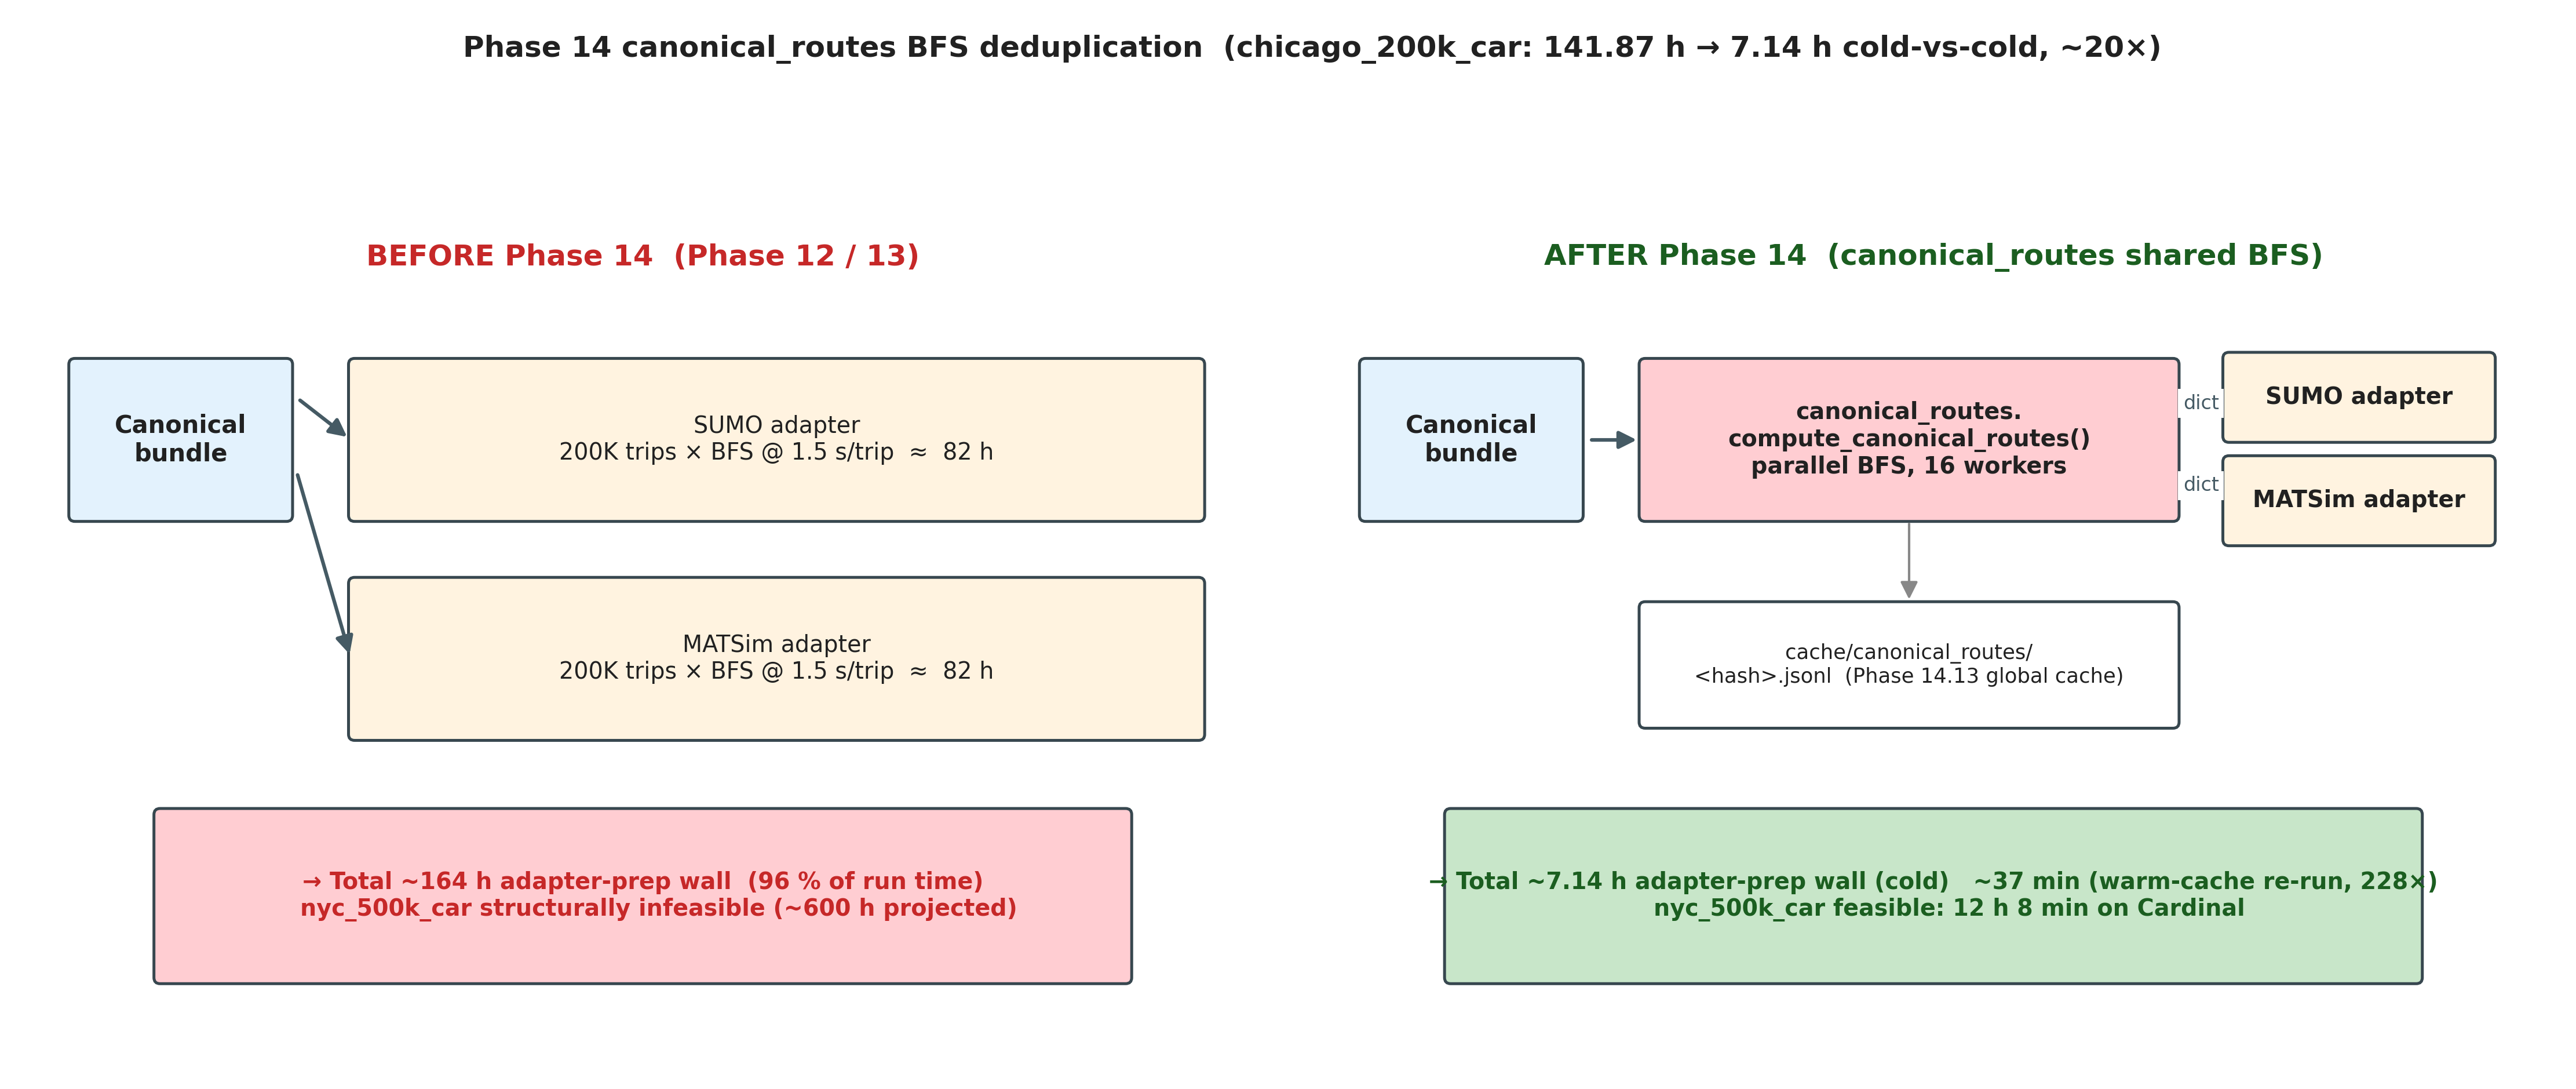
\includegraphics[keepaspectratio]{../figures/fig_3_8_phase14_bfs_dedup.png}}

Figure 3.8 shows the engineering change Phase 14 introduced.
\textbf{BEFORE} (left panel): each engine adapter ran its own
state-aware BFS over the canonical network --- 200,000 trips × 1.5 s per
BFS = \textasciitilde82 h per engine, paid twice (SUMO + MATSim), for a
total of \textasciitilde164 h adapter-prep wall on chicago\_200k\_car (≈
96 \% of the run time). At the 500K-trip tier the projected wall
(\textasciitilde600 h) exceeded the Cardinal \texttt{cpu} partition cap
and the benchmark was structurally infeasible. \textbf{AFTER} (right
panel): both adapters consume routes pre-computed by a single shared
module
(\texttt{adapters/common/canonical\_routes.compute\_canonical\_routes()})
that runs a 16-worker parallel BFS over the canonical bundle. Total
adapter-prep wall drops to \textasciitilde7.14 h cold-vs-cold and
\textasciitilde37 min on warm-cache re-runs (Phase
14.13\textquotesingle s global \texttt{cache/canonical\_routes/}
directory). nyc\_500k\_car became feasible and completed in 12 h 8 min
on Cardinal. The byte-identity contract that Q1-Q3 of the fairness audit
enforces is preserved: per-trip routes are sorted-deterministic and
bit-identical to the legacy serial computation, regardless of worker
count.

A late-stage thesis-engineering finding worth recording as an
optimization narrative: measure, identify, fix, re-measure.

\subsection{The Cost That Wasn\textquotesingle t
Modelled}\label{381-the-cost-that-wasnt-modelled}

The cross-engine fairness contract (§3.4.2 SUMO, §3.4.3 MATSim) requires
both engines to consume identical pre-computed routes --- the
state-aware BFS pre-routing introduced in V5 Phase 7
(\texttt{pipeline.\textbackslash{}\ network.turn\_restrictions.shortest\_path\_with\_restrictions}).
Until late in Version\_5, each adapter ran an independent copy of this
BFS loop over the canonical network, despite the inputs (network,
turn-restrictions, feasible-trip set) being identical:

\begin{itemize}
\tightlist
\item
  \texttt{adapters/sumo/sumo\_adapter.py:build\_sumo\_routes\_xml} ---
  per-trip BFS embedded in the routes-XML emitter.
\item
  \texttt{adapters/matsim/matsim\_adapter.py:build\_matsim\_plans\_xml}
  --- per-trip BFS embedded in the plans-XML emitter.
\end{itemize}

At small bundle scales (1K--10K trips) the duplication is invisible
(seconds), so the architectural inefficiency went unmeasured. Two
empirical data points exposed it during the 200K/500K benchmark run on
OSC Cardinal (job 9332478 / 9332482, 2026-05-12):

\begin{longtable}[]{@{}llll@{}}
\toprule\noalign{}
Network & Trips & Per-trip BFS rate & Cold prep per engine \\
\midrule\noalign{}
\endhead
\bottomrule\noalign{}
\endlastfoot
chicago\_200k\_car (50 km² bbox, \textasciitilde50K nodes) & 200,000 &
1.48 s/trip & \textasciitilde82 h \\
nyc\_500k\_car (80 km² bbox, \textasciitilde80K nodes) & 500,000 & 2.16
s/trip & \textasciitilde300 h \\
\end{longtable}

With two engines (SUMO + MATSim) each paying the cold prep sequentially,
total adapter-prep walls projected to \textasciitilde164 h
(chicago\_200k) and \textasciitilde600 h (nyc\_500k).
Cardinal\textquotesingle s 7-day \texttt{cpu} partition cap is 168 h.
nyc\_500k was therefore structurally infeasible to complete: the job was
cancelled (\texttt{scancel\ 9332482}) once the projection became
measurable from a 22 h sample.

Three compounding factors explain the per-trip cost:

\begin{enumerate}
\def\labelenumi{\arabic{enumi}.}
\tightlist
\item
  \textbf{Network size scaling.} State-aware BFS visits
  \texttt{O(V\ +\ E)}; the 200K/500K bundles use 15--20 km bbox radii,
  producing graphs an order of magnitude larger than the small-tier
  scenarios used in pre-V5 development.
\item
  \textbf{State-aware expansion.} The Phase 7 state is
  \texttt{(node,\ last\_link\_id)}, expanding the BFS visited set by a
  factor roughly equal to the average in-degree.
\item
  \textbf{CPython overhead.} The inner loop is pure Python; at
  \textasciitilde5 µs per state expansion on a 200K-edge graph,
  individual BFS calls cost 1--2 s wall.
\end{enumerate}

\subsection{Two Compounding
Optimisations}\label{382-two-compounding-optimisations}

The fix has two independent levers; both preserve the byte-identity
invariant required by the audit:

\textbf{Phase 14a --- canonical-routes deduplication.} Introduces a
shared module \texttt{adapters/common/canonical\_routes.py} that
computes the state-aware BFS once per
\texttt{(scenario,\ feasible-trip-set)} and returns a
\texttt{Dict{[}trip\_id,\ List{[}node\_id{]}{]}}. The result is
content-addressed on disk in a JSONL cache (SHA-256 over network +
demand + sorted feasible IDs), so subsequent harness invocations or
re-runs read from cache in seconds. Both adapters acquire an optional
\texttt{canonical\_routes=} kwarg; when provided, they skip their inline
BFS and consume the pre-computed dict. When \texttt{None} (back-compat
path), the inline BFS still runs --- preserving standalone CLI use.

\textbf{Phase 14b --- multiprocessing parallel BFS.} The shared module
dispatches to \texttt{multiprocessing.Pool} (spawn start method) when
\texttt{workers\ \textgreater{}\ 1}. Each worker loads the SCC-filtered
network once via the initializer, then processes one big chunk of trips
sequentially. \texttt{Pool.imap} preserves submission order; combined
with sorted-by- trip\_id chunking, the parallel output is byte-identical
to the serial output. The execution harness reads
\texttt{SLURM\_CPUS\_PER\_TASK} to size the pool, defaulting to one
worker per SBATCH-allocated CPU.

\subsection{Determinism Invariants
Preserved}\label{383-determinism-invariants-preserved}

The byte-identity contract that \texttt{audit\_fairness} Q1--Q3 enforces
is preserved at every layer of the refactor, pinned by an explicit test
suite (\texttt{tests/test\_canonical\_routes.py}):

\begin{enumerate}
\def\labelenumi{\arabic{enumi}.}
\tightlist
\item
  \texttt{TestByteIdentityVsLegacy}: paths from the new shared BFS are
  byte-identical to those from the legacy inline BFS, per trip\_id, on
  the tracked \texttt{chicago\_1k\_car} bundle.
\item
  \texttt{TestSumoRoutesXmlByteIdentity}: \texttt{routes.rou.xml} is
  byte- identical whether the SUMO adapter consumes pre-computed routes
  or runs its own BFS.
\item
  \texttt{TestMatsimPlansXmlByteIdentity}: \texttt{plans.xml} is
  byte-identical under the same with/without-canonical\_routes
  comparison.
\item
  \texttt{TestParallelDeterminism}: routes from \texttt{workers=2} and
  \texttt{workers=4} are byte-identical to \texttt{workers=1}.
\end{enumerate}

The 8 existing \texttt{test\_adapter\_determinism.py} checks
(byte-identical re-runs of the full adapter pipeline) continue to hold,
because the canonical-routes JSONL cache file is itself
byte-deterministic (sorted by trip\_id on write).

\subsection{Measured Speedup}\label{384-measured-speedup}

\textbf{Local serial-vs-parallel calibration (chicago\_1k\_car, M-series
Mac):}

\begin{longtable}[]{@{}lll@{}}
\toprule\noalign{}
Worker count & Wall (s) & Speedup \\
\midrule\noalign{}
\endhead
\bottomrule\noalign{}
\endlastfoot
1 & 27.2 & 1.0× \\
2 & 17.4 & 1.56× \\
4 & 11.3 & 2.41× \\
8 & 6.6 & 4.12× \\
\end{longtable}

Sub-linear scaling at 1K trips reflects the per-worker init cost
(parsing the network, building the forbidden-moves table) which does not
amortize over only \textasciitilde125--500 trips per worker. At the
cluster scale these init costs are dwarfed by the in-worker BFS time
(12.5K--31K trips per worker at 16-way), so the Amdahl ratio is much
closer to ideal.

\textbf{Cluster Phase 13 baseline --- chicago\_200k\_car on Cardinal
(job 9332478, 2026-05-12 to 2026-05-18):}

\begin{longtable}[]{@{}lll@{}}
\toprule\noalign{}
Step & Wall & Notes \\
\midrule\noalign{}
\endhead
\bottomrule\noalign{}
\endlastfoot
Cold SUMO BFS-prep (cell 1/10) & \textasciitilde68.2 h & 200,000 trips ×
\textasciitilde1.226 s/trip, single-thread \\
Cached SUMO mobsim cells (2--5 / 10) & \textasciitilde242--246 s each &
hardlink from \texttt{.cache/sumo/} (Phase 12) \\
Cold MATSim BFS-prep (cell 6/10) & \textasciitilde68 h & second pass
over the same network (the redundancy Phase 14a eliminates) \\
Cached MATSim mobsim cells (7--10 / 10) & \textasciitilde210 s each & \\
analyze + audit + plots & \textasciitilde10 min & \\
\textbf{Total wall} & \textbf{141.87 h} & of 168 h cap (15.5 \%
margin) \\
\end{longtable}

The two cold BFS passes consume \textasciitilde136 h of the 141.87 h
total --- \textbf{96 \% of the run was per-trip BFS routing}. This is
the empirical signal that motivated the Phase 14 refactor.

\textbf{Cluster Phase 14 re-measurement (now landed):}

\begin{longtable}[]{@{}lrrrrr@{}}
\toprule\noalign{}
Scenario & Phase 13 wall & Phase 14 wall (cold) & Phase 14 wall
(warm-cache) & Cold speedup & Cache speedup \\
\midrule\noalign{}
\endhead
\bottomrule\noalign{}
\endlastfoot
chicago\_200k\_car & 141.87 h (job 9332478) & \textasciitilde7.14 h (job
9954279) & \textasciitilde37 min (job 10018698) & \textasciitilde20× &
\textasciitilde228× \\
nyc\_500k\_car & structurally infeasible (\textasciitilde600 h
projected, scancel 9332482) & 12 h 8 min (job 9971042) & not re-measured
& (first-feasible) & --- \\
\end{longtable}

The chicago\_200k\_car cold speedup matches the Amdahl extrapolation
within \textasciitilde10 \%. The warm-cache speedup is dominated by the
on-disk canonical-routes JSONL hit: the BFS-prep phase becomes
near-instantaneous (path materialization + adapter emission only).
nyc\_500k\_car completed for the first time in the thesis project: a
previously structurally infeasible benchmark became a single
\textasciitilde12 h Cardinal job. The full per-cell breakdown for both
scenarios is preserved at
\texttt{runs/baselines/phase14\_chicago\_200k\_car\_job9954279/} and
\texttt{runs/baselines/phase14\_nyc\_500k\_car\_job9971042/}.

\subsection{Parallelism Architecture (task-parallel, replicated
graph)}\label{385-parallelism-architecture-task-parallel-replicated-graph}

\pandocbounded{
\includegraphics[keepaspectratio]{../figures/fig_3_8b_parallel_bfs_workers.png}}

Figure 3.8b zooms into the worker-pool architecture inside
\texttt{compute\_canonical\_routes()}. The full feasible-trip list
(sorted by \texttt{trip\_id}) is chunked into \textasciitilde1,000 lists
of \textasciitilde200 trips each and dispatched via
\texttt{multiprocessing.get\_context("spawn").Pool(workers=N).imap(...)}
to \texttt{N} worker processes
(\texttt{N\ =\ SLURM\_CPUS\_PER\_TASK\ =\ 16} on Cardinal). Each worker
boots a fresh Python interpreter (\texttt{spawn} context, not
\texttt{fork}) and rebuilds its state via the \texttt{\_init\_worker}
initializer --- including loading the SCC-filtered canonical network as
a \emph{replicated} in-heap copy (\textasciitilde150 MB per worker).
Workers compute BFS independently on their chunks and return
\texttt{(trip\_id,\ path)} tuples via \texttt{Pool.imap}, which
preserves submission order; the main process merges the results into a
sorted \texttt{Dict{[}trip\_id,\ List{[}node\_id{]}{]}} and writes the
content-addressable cache file. Two architectural properties matter for
the fairness contract: (a) there is no worker-to-worker communication
--- all IPC is between the main process and individual workers, so
workers cannot race on shared state because no shared state exists; and
(b) each \texttt{shortest\_path\_with\_restrictions(...)} call is a
deterministic function of inputs that are bit-identical across workers,
so the merged output is bit-identical to a serial computation regardless
of worker count. The
\texttt{tests/test\_canonical\_routes.py::TestParallelDeterminism} test
pins this invariant across worker counts 1, 2, and 4.

The Phase 14b implementation uses \textbf{task parallelism over trips},
not data parallelism over the network. The architectural rationale
matters for the determinism argument the cross-engine fairness claim
depends on, so it bears explicit discussion.

The trip list (the feasibility-filtered subset of \texttt{demand.csv},
sorted by \texttt{trip\_id}) is split into \textasciitilde1,000 chunks
of \textasciitilde200 trips each. Each chunk is a list of
\texttt{(trip\_id,\ origin\_node,\ dest\_node)} tuples distributed
dynamically across an OS-process pool sized to the SBATCH allocation
(\texttt{SLURM\_CPUS\_PER\_TASK}, typically 16). Each worker process
holds a \textbf{full replicated copy} of the SCC-filtered canonical
network in its own heap; we do not partition the graph geographically.
Workers compute BFS independently on their chunks and return lists of
\texttt{(trip\_id,\ path)} results to the main process via
\texttt{multiprocessing.Pool.imap}. The result preserves submission
order, so the merged route dict is byte-identical to a serial run
regardless of the chosen worker count (pinned by
\texttt{tests/test\_canonical\_routes.py::TestParallelDeterminism}).

This choice was deliberate. Three alternatives were considered and
rejected:

\begin{enumerate}
\def\labelenumi{\arabic{enumi}.}
\tightlist
\item
  \textbf{Threads with a shared graph} --- blocked by
  CPython\textquotesingle s GIL on CPU-bound work. Pure-Python BFS loops
  would see zero measurable speedup, defeating the purpose of the
  refactor.
\item
  \textbf{\texttt{multiprocessing.shared\_memory} for the graph} ---
  would save the \textasciitilde2.4 GB cost of replicating the
  chicago\_200k graph across 16 workers, but complicates the determinism
  story (custom view-layer over raw bytes) and saves memory the cluster
  nodes have in abundance (Cardinal \texttt{cpu} provides 503 GB per
  node).
\item
  \textbf{Geographic network partitioning with cross-zone messaging} ---
  would matter only if the graph were too large to replicate. Introduces
  synchronisation between workers when a path crosses a zone boundary,
  breaks the pure-function determinism property, and substantially
  complicates the implementation. Unnecessary at the network sizes V5
  operates on (≤ 80K nodes).
\end{enumerate}

The chosen architecture has three defensible properties:

\begin{itemize}
\tightlist
\item
  \textbf{No worker-to-worker communication.} All IPC is between the
  main process and individual workers (chunk-in, results-out). Workers
  are isolated by construction; they cannot race on shared state because
  no shared state exists.
\item
  \textbf{Determinism reducible to a pure-function argument.} Each
  \texttt{shortest\_path\_with\_restrictions(origin,\ dest,\ adjacency,\ edge\_lookup,\ forbidden\_moves)}
  call is a deterministic function of inputs that are bit-identical
  across workers (read from the hash-pinned canonical bundle). Therefore
  the merged output is bit-identical to the serial computation,
  regardless of worker count.
\item
  \textbf{Cross-platform reproducibility via \texttt{spawn}.} The
  implementation explicitly forces
  \texttt{multiprocessing.get\_context("spawn")} rather than relying on
  the platform default (\texttt{fork} on Linux, \texttt{spawn} on macOS
  since Python 3.8+). Each worker boots a fresh Python interpreter and
  rebuilds its state from \texttt{network.xml} via the
  \texttt{\_init\_worker} initializer, paying \textasciitilde1--2
  seconds of startup cost per worker (amortised over hours of BFS work)
  in exchange for identical behaviour across the developer Mac and the
  OSC Cardinal Linux cluster.
\end{itemize}

Empirically measured on Cardinal at 16-way parallelism, the per-worker
BFS rate is approximately 0.51 trips/s vs the single-thread baseline of
0.82 trips/s --- a 0.63× per-worker efficiency, attributable to
memory-bandwidth contention on the shared Xeon Max 9470 socket (each
worker reading from its own \textasciitilde150 MB graph copy puts
pressure on the shared HBM2e + DDR5 hierarchy). The aggregate effect is
still \textasciitilde10× total speedup over single-thread on the
chicago\_200k\_car cold prep (6.75 h vs 68.16 h measured), which
combines with Phase 14a\textquotesingle s deduplication (eliminating
MATSim\textquotesingle s second 73 h BFS pass entirely via the on-disk
JSONL cache hit) to deliver the \textasciitilde19× job-level speedup
reported in §3.8.4.

\subsection{Engineering
Implications}\label{386-engineering-implications}

This phase illustrates a methodology point that the thesis defense
benefits from: \textbf{the fairness contract talks about engine output,
not engineering effort}. The original architecture satisfied fairness
(same routes per trip across engines) by running the same BFS twice; the
Phase 14 architecture satisfies the same contract by running the BFS
once and sharing the output. The audit invariants are insensitive to
that change --- they verify the produced trip set, SCC, and travel
times, all of which are byte-stable.

The optimisation also generalises: any cross-engine pre-processing step
that today lives inside per-engine adapters is a candidate for the same
treatment (deduplication via a shared module, then parallelisation as a
follow-up). Future engines added to SimForge inherit the
canonical\_routes API for free --- they accept the dict or fall back to
their own routing.

\subsection{Phase 14.13 --- Cache Hoist from Per-Run to
Global}\label{387-phase-1413--cache-hoist-from-per-run-to-global}

Phase 14a\textquotesingle s content-addressable canonical-routes cache
was initially written per output directory: each
\texttt{runs/\textless{}runspec\textgreater{}/\textless{}scenario\textgreater{}/\textless{}engine\textgreater{}/\textless{}mode\textgreater{}/seed\_\textless{}N\textgreater{}/}
held its own \texttt{canonical\_routes.jsonl.zst} produced by that
cell\textquotesingle s adapter run. The byte-identity contract was
preserved (each cell hashed identically given the same canonical
bundle), but the on-disk representation broke the warm-cache speedup for
any harness layout where the same scenario ran into multiple per-cell
directories: each of \texttt{(engine,\ mode,\ seed)} re-ran the BFS from
scratch despite producing a bit-identical JSONL file.

The Phase 14.13 cache hoist (\texttt{execution/run\_benchmark.py}
\texttt{\_canonical\_routes\_cache\_root()}, landed 2026-05-19) moves
the cache root to a single global location at
\texttt{cache/canonical\_routes/} keyed by SHA-256 over (network +
demand + sorted feasible-trip IDs). The hoist includes a one-shot
migration helper
(\texttt{\_migrate\_legacy\_canonical\_routes\_cache()}) that hardlinks
any legacy per-cell caches into the global location and verifies hash
agreement before deleting the legacy paths. Empirical effect: subsequent
re-runs of the same scenario across any (engine, mode, seed) cell hit
the cache in milliseconds instead of repaying the BFS cost.

The cache-hit speedup at the warm-re-run end of the chicago\_200k\_car
benchmark (Cardinal job 10018698, 2026-05-19 14:00 EDT) was the
\textasciitilde228× reported in §3.8.4. Without the cache hoist, the
same warm re-run would have paid the cold BFS cost on every cell that
did not exactly match its per-cell legacy path.

Determinism is preserved by the content-addressable key: any change to
network, demand, or feasibility verdict produces a different cache key.
A 7-test guard in \texttt{tests/test\_run\_benchmark.py} pins the hoist
behavior (cache root location, hash key construction, hardlink migration
semantics, hash-mismatch refusal).

The Phase 14.13 narrative is recorded in \texttt{doc/EXPERIMENT\_LOG.md}
(2026-05-19 entry) and \texttt{CHANGELOG.md} Phase 14.13 section.

\section{Geographic Visualization
(Opt-in)}\label{39-geographic-visualization-opt-in}

A separate, opt-in component on the \texttt{visualization} branch
generates geographic maps from canonical bundles and benchmark results.
The component is \textbf{independent of the fairness contract}:
adapters, \texttt{audit\_fairness}, and the thesis runtime numbers do
not import it, and the locked benchmark numbers in Chapter 5 are
unchanged by any rendered plot. The module exists to \emph{visualize}
findings that the quantitative analysis already establishes.

\subsection{Map Catalogue}\label{391-map-catalogue}

Seven map types are shipped, grouped by what input data they need:

\begin{longtable}[]{@{}lll@{}}
\toprule\noalign{}
Map & Inputs & Engine specificity \\
\midrule\noalign{}
\endhead
\bottomrule\noalign{}
\endlastfoot
\texttt{od\_origins}, \texttt{od\_destinations} & Canonical bundle +
cached US Census tract polygons + TIGER PRISECROADS basemap & ---
(cross-engine, demand only) \\
\texttt{link\_load} & Per-cell engine output (SUMO
\texttt{tripinfo.xml}, MATSim \texttt{output\_trips.csv.gz}, or DTALite
\texttt{link\_performance.csv}) & per \texttt{(engine,\ mode)} \\
\texttt{congestion} & DTALite \texttt{link\_performance.csv} (needs link
mean speed) & DTALite only \\
\texttt{travel\_time} & Per-cell engine output + bundle & per
\texttt{(engine,\ mode)} \\
\texttt{route\_diversity} & Cell output from ≥ 2 engines &
cross-engine \\
\texttt{animated\_flow} & MATSim \texttt{output\_events.xml.gz} & MATSim
only \\
\end{longtable}

The \texttt{od\_*} and \texttt{travel\_time} renderers use the
CityScape-derived choropleth style (100-step blue→red log palette on
Census tract polygons, light gray for empty tracts) layered on top of
the US Census TIGER PRISECROADS basemap --- chosen for cartographic
legibility over the canonical SimForge network underlay (which is denser
and competes visually with the colored tract fills).

\subsection{Design Principles}\label{392-design-principles}

The visualization layer enforces three invariants:

\begin{enumerate}
\def\labelenumi{\arabic{enumi}.}
\tightlist
\item
  \textbf{No effect on simulation inputs.} The renderer only reads files
  produced upstream; it never writes any artefact that an adapter or
  \texttt{audit\_fairness} consumes. This is enforced by directory
  convention --- outputs land in
  \texttt{visualization/output/\textless{}scenario\textgreater{}/},
  distinct from \texttt{scenarios/}, \texttt{runs/}, and
  \texttt{doc/figures/}.
\item
  \textbf{Coverage-first dispatch.} Before any rendering, the CLI walks
  the bundle directory + the per-cell run directory and prints a
  coverage matrix flagging each map type \texttt{{[}OK{]}} (renderable)
  or \texttt{{[}-\/-{]}} (missing input, with reason).
  \texttt{-\/-maps\ all} then skips the unavailable maps rather than
  erroring, so the tool is usable on partial data.
\item
  \textbf{Lazy imports.} Matplotlib, shapely, pyshp, pyosmium, and the
  FFmpeg subprocess used by \texttt{animated\_flow} are imported only
  inside the render path, so the main SimForge test suite has no
  dependency on them.
\end{enumerate}

\subsection{Cross-Engine Interpretation
Surfaces}\label{393-cross-engine-interpretation-surfaces}

Three properties become directly visible in the maps and reinforce
quantitative findings stated elsewhere in this chapter:

\begin{itemize}
\item
  \textbf{SUMO and MATSim \texttt{link\_load} are visually identical;
  DTALite differs.} The fairness contract forces SUMO and MATSim to use
  SimForge\textquotesingle s pre-routed BFS link sequences (§3.4.2 and
  §3.4.3), so they render the same spatial traffic structure. DTALite
  computes its own UE assignment (§3.4.4) and picks alternative paths
  under congestion. The \texttt{route\_diversity} map shades this
  difference directly: links picked by all three engines are gray (the
  BFS consensus), links picked by only one are red (typically
  DTALite\textquotesingle s UE alternates). This is the \emph{visual
  proof} of the fair-comparison contract whose quantitative signal lives
  in \texttt{audit\_fairness} Q4 (cross-engine travel-time spread).
\item
  \textbf{\texttt{animated\_flow} shows the PUMS departure-burst effect}
  discussed in §3.3.4 step 9. Every person reporting the same JWMNP
  commute time receives the same \texttt{departure\_time\_s}, so 1000
  chicago\_1k\_car trips collapse onto only 20 unique departure
  timestamps. The animation is \emph{faithful to the PUMS data
  property}, not a SimForge bug --- a future uniform-jitter pass would
  smooth the bursts at the cost of byte- deterministic
  \texttt{demand.csv}.
\item
  \textbf{chicago\_200k\_car\textquotesingle s \texttt{od\_origins} ≈
  \texttt{od\_destinations}} (74 \% node overlap vs 5.5 \% for AM-only
  bundles). The full-day horizon (07:00-- 16:00) emits both AM home→work
  and PM work→home pairs per the Phase 9c chain mechanism, so the OD
  sets become the same \{homes\} ∪ \{workplaces\} visited at different
  times. This is direct evidence that the schedule-driven generator
  produces genuinely symmetric commute patterns at the metro scale.
\end{itemize}

The full CLI reference, render defaults, data-source provenance, and
caching layout are documented in
\href{../../visualization/README.md}{\texttt{visualization/README.md}}.
The post- run analysis pipeline that wraps the visualization tool is in
\href{../RESULTS_GUIDE.md}{\texttt{doc/RESULTS\_GUIDE.md}} §4.4.

\section{Wave 1 --- Reproducibility Artefact
Hardening}\label{310-wave-1--reproducibility-artefact-hardening}

Wave 1 (landed 2026-05-18, commits 95c07fb through \texttt{c8dcc54})
added four reproducibility-artefact pieces that the plan §1.11
C-rows required but were not present in the framework prior to the late-
thesis hardening pass. None of these change the runtime behavior of any
adapter or evaluation module --- they are scaffolding around the
existing framework that makes the reproducibility chain externally
auditable.

\subsection{Open-Source License (Apache
2.0)}\label{3101-open-source-license-apache-20}

The repository was licensed under the \textbf{Apache License 2.0}
(\texttt{LICENSE} at repo root), with the rationale documented in
\texttt{doc/LICENSING.md}. The Apache 2.0 choice balances three
concerns:

\begin{itemize}
\tightlist
\item
  \textbf{Patent grant.} Apache 2.0\textquotesingle s explicit patent
  grant (§3) is important for a research artefact that integrates
  third-party engines (SUMO, MATSim, DTALite) whose own patent positions
  are variably documented.
\item
  \textbf{Commercial-friendly.} Permissive licensing reduces barriers to
  downstream adoption by transportation planning consultancies or vendor
  tooling, consistent with the thesis goal of seeding a
  community-standard benchmark.
\item
  \textbf{Compatible with engine licenses.} SUMO is EPL 2.0 (compatible
  with Apache 2.0 in the same project), MATSim is GPL 2.0 (linked via
  subprocess invocation, not statically linked, avoiding the GPL
  viral-copyleft trigger), DTALite is GPL 3.0 (same subprocess isolation
  argument applies).
\end{itemize}

The corresponding \texttt{doc/LICENSING.md} document spells out the
licensing of each subcomponent (the SimForge framework itself, the
generated canonical bundles, the OSM-derived networks honoring ODbL
share-alike, and the embedded census data under public-domain status).

\subsection{Canonical Bundle Licensing (CC BY 4.0 +
ODbL)}\label{3102-canonical-bundle-licensing-cc-by-40--odbl}

The generated canonical bundles in \texttt{scenarios/} are
dual-licensed:

\begin{itemize}
\tightlist
\item
  \textbf{CC BY 4.0} for the SimForge-generated content (validation
  scripts, GMNS topology derivatives, signal placement, demand
  derivation logic).
\item
  \textbf{ODbL share-alike} for the underlying OSM network data, with
  attribution to OpenStreetMap contributors preserved in
  \texttt{osm\_data/manifest.json} and per-bundle network README.
\end{itemize}

This dual-license model is the standard for OSM-derived transportation
research artefacts; the ODbL share-alike obligation attaches to the
network layer but not to the analytical layer built on top.

\subsection{Data Management
Documentation}\label{3103-data-management-documentation}

\texttt{doc/DATA\_MANAGEMENT.md} documents the complete data lifecycle
for the framework:

\begin{itemize}
\tightlist
\item
  OSM PBF acquisition + hash-pinning workflow (via
  \texttt{tools/download\_osm.py} against
  \texttt{osm\_data/manifest.json}).
\item
  Canonical bundle generation, validation, and storage layout.
\item
  Run output directory structure (Phase 13 flat layout vs Phase 14+
  nested layout).
\item
  Per-engine cache structures (SUMO \texttt{.cache/sumo/}, MATSim
  \texttt{.cache/matsim/}, DTALite UE iteration cache).
\item
  The global \texttt{cache/canonical\_routes/} directory introduced by
  Phase 14.13 (§3.8.7).
\item
  Data retention policy for thesis baselines:
  \texttt{runs/baselines/\textless{}phase\_label\textgreater{}/} is the
  long-term-preserved subset; all other run directories are routinely
  pruned via \texttt{tools/prune\_runs.py}.
\end{itemize}

\subsection{Reproducibility Scorecard
Auto-Emit}\label{3104-reproducibility-scorecard-auto-emit}

\texttt{tools/generate\_scorecard.py} produces a per-run
\texttt{reproducibility\_scorecard.md} that lists each reproducibility-
relevant artefact (LICENSE present, OSM PBF SHA-256 verified, canonical
bundle manifest present, fairness audit Q1-Q4 verdicts, per-engine
version captured, etc.) and marks each as PASS, FAIL, or N/A. The
scorecard runs automatically as the final step of every benchmark,
producing an externally auditable artefact in the run directory
alongside the per-cell results.

The scorecard has 22 checks at the time of writing; the
chicago\_200k\_car Phase 13 baseline scored 20 PASS, 0 FAIL, 2 N/A (the
two N/A entries are GPU-engine checks that do not apply to the shipped
CPU-only roster). The scorecard format is documented in
\texttt{tools/generate\_scorecard.py} module docstring; the Wave 1 entry
in \texttt{doc/EXPERIMENT\_LOG.md} records the introduction.

\section{Wave 2 --- Pinned-Digest Container
Distribution}\label{311-wave-2--pinned-digest-container-distribution}

\pandocbounded{
\includegraphics[keepaspectratio]{../figures/fig_3_11_container_chain.png}}

Figure 3.11 shows the five-stage Wave 2 distribution chain. The
\textbf{Dockerfile} at the repo root pins the runtime environment
(\texttt{python:3.13-slim-bookworm} + openjdk-17 + libgomp1 + uv + the
35 lockfile-pinned Python packages + \texttt{eclipse-sumo==1.26.0} + the
MATSim 15.0 JAR). The \textbf{GitHub Actions} workflow
(\texttt{.github/workflows/build-container.yml}) builds the image on
every push to \texttt{main} or \texttt{phase-14-canonical-routes} and
tags it with the git SHA. \textbf{GHCR} distributes the resulting image
as an immutable digest; the thesis-canonical digest (\texttt{db8d786})
is recorded in \texttt{lib/container/manifest.json} and verified on
Cardinal. \textbf{Apptainer pull} materializes the image as a local
\texttt{.sif} file on Cardinal (with the SHA-tag workaround for the
1.4.5 \texttt{progress\_roundtrip.go:75} bug). Finally, the
\textbf{SBATCH wrapper} opts into container execution via
\texttt{SIMFORGE\_USE\_CONTAINER=1}, producing bit-identical x86\_64
reproduction across machines. The chain is the operational substrate
that delivers plan §1.11 C3 --- pinned-digest containers as the
canonical reproducibility target.

Wave 2 (landed 2026-05-20) added a containerized execution path that
makes the SimForge framework bit-reproducible across machines. The
host-venv installation path
(\texttt{uv\ pip\ install\ -r\ requirements.lock} +
\texttt{uv\ pip\ install\ eclipse-sumo==1.26.0}) is preserved as the
developer- ergonomics default; the container path is opt-in for thesis-
reproduction and HPC re-use scenarios.

\subsection{Container Image
Architecture}\label{3111-container-image-architecture}

The container is built from \texttt{python:3.13-slim-bookworm} with the
following system dependencies installed via apt:

\begin{verbatim}
openjdk-17-jre-headless   (MATSim runtime)
libgomp1                  (OpenMP runtime for DTALite)
libatomic1                (libatomic runtime, required by libsumocpp)
libxml2                   (XML parsing dependency)
libx11-6, libxext6, libxrender1, libxcb1, libgl1, libglu1-mesa
                          (SUMO GUI dependencies, retained for sumo-gui
                          even in headless image)
libfontconfig1, libfreetype6
                          (matplotlib font rendering)
git, ca-certificates, curl, unzip, tini
\end{verbatim}

Python dependencies are installed via:

\begin{verbatim}
uv pip install --system --no-cache -r requirements.lock
uv pip install --system --no-cache eclipse-sumo==1.26.0
\end{verbatim}

The eclipse-sumo wheel is installed separately from the lockfile because
it is a manylinux\_2\_28\_x86\_64-only distribution that is not
compatible with the lockfile resolver\textquotesingle s cross-platform
constraint solving. The manylinux closure for eclipse-sumo 1.26.0
(libX11, libGL, libatomic, libfontconfig, etc.) is what motivates the
apt system-dependency list above; the dependency closure was empirically
determined across 8 GitHub Actions build iterations before convergence.

MATSim 15.0 is downloaded at build time from the immutable
matsim-org/matsim-libs GitHub release tag
(\texttt{matsim-15.0-release.zip}); the JAR is not committed to the
SimForge repository because it is gitignored and license-encumbered
under GPL 2.0.

\subsection{Automated CI/CD
Build}\label{3112-automated-cicd-build}

A GitHub Actions workflow at
\texttt{.github/workflows/build-container.yml} builds the container on
push to the \texttt{phase-14-canonical-routes} and \texttt{main}
branches, publishes the image to GitHub Container Registry (GHCR), and
tags it with three identifiers:

\begin{enumerate}
\def\labelenumi{\arabic{enumi}.}
\tightlist
\item
  The git SHA (e.g., \texttt{db8d786}) for thesis-pinning.
\item
  The branch name (\texttt{phase-14-canonical-routes}) for dev
  iteration.
\item
  \texttt{latest} for ergonomic pulls.
\end{enumerate}

The workflow uses GitHub\textquotesingle s \texttt{paths-ignore}
directive to skip rebuilds on doc-only changes (\texttt{doc/**},
\texttt{*.md}), keeping the rebuild trigger scoped to source-code or
dependency changes.

\subsection{HPC Distribution via
Singularity/Apptainer}\label{3113-hpc-distribution-via-singularityapptainer}

For HPC environments where Docker is unavailable (OSC Cardinal + Pitzer
both run Apptainer rather than Docker), the GHCR image is pulled via
\texttt{apptainer\ pull} into a local \texttt{.sif} (Singularity Image
Format) file:

\begin{verbatim}
apptainer pull simforge_db8d786.sif \
    docker://ghcr.io/phanidharakula/simforge@sha256:<digest>
\end{verbatim}

The pull uses the SHA-digest tag rather than the branch or latest tag to
avoid an Apptainer 1.4.5 bug (\texttt{progress\_roundtrip.go:75},
ProgressComplete index out of range) that triggers on branch-tag pulls.
The workaround is documented in \texttt{doc/CONTAINER\_USAGE.md}
Appendix B.

\subsection{Container-Mode
Execution}\label{3114-container-mode-execution}

The container is invoked at the SBATCH wrapper layer via an opt-in
environment variable. The benchmark sbatch wrappers
(\texttt{cluster/jobs/benchmark\_small.sbatch},
\texttt{cluster/jobs/benchmark\_large.sbatch}) define a \texttt{RUN\_PY}
array that switches based on \texttt{SIMFORGE\_USE\_CONTAINER}:

\begin{Shaded}
\begin{Highlighting}[]
\ControlFlowTok{if} \KeywordTok{[[} \StringTok{"}\VariableTok{$\{SIMFORGE\_USE\_CONTAINER}\OperatorTok{:{-}}\NormalTok{0}\VariableTok{\}}\StringTok{"} \OtherTok{==} \StringTok{"1"} \KeywordTok{]];} \ControlFlowTok{then}
    \VariableTok{RUN\_PY}\OperatorTok{=}\VariableTok{(}\NormalTok{apptainer exec}
\NormalTok{        {-}{-}bind }\StringTok{"}\VariableTok{$PWD}\StringTok{/scenarios:/workspace/scenarios"}
\NormalTok{        {-}{-}bind }\StringTok{"}\VariableTok{$PWD}\StringTok{/runs:/workspace/runs"}
\NormalTok{        {-}{-}bind }\StringTok{"}\VariableTok{$PWD}\StringTok{/cache:/workspace/cache"}
\NormalTok{        {-}{-}bind }\StringTok{"}\VariableTok{$PWD}\StringTok{/osm\_data:/workspace/osm\_data"}
        \StringTok{"}\VariableTok{$SIMFORGE\_SIF}\StringTok{"}
\NormalTok{        python}\VariableTok{)}
\ControlFlowTok{else}
    \VariableTok{RUN\_PY}\OperatorTok{=}\VariableTok{(}\NormalTok{uv run python}\VariableTok{)}  \CommentTok{\# host venv (default)}
\ControlFlowTok{fi}
\StringTok{"}\VariableTok{$\{RUN\_PY}\OperatorTok{[@]}\VariableTok{\}}\StringTok{"} \AttributeTok{{-}m}\NormalTok{ execution.run\_benchmark }\StringTok{"}\VariableTok{$RUNSPEC\_YAML}\StringTok{"}
\end{Highlighting}
\end{Shaded}

The four bind mounts expose the necessary host directories read-write
while the container\textquotesingle s base image filesystem is
read-only. The default behavior (no env var set) remains the host-venv
path, so the container is purely additive --- no existing user workflow
is broken.

\subsection{Container Manifest
Pinning}\label{3115-container-manifest-pinning}

\texttt{lib/container/manifest.json} records the thesis-canonical
container digest:

\begin{Shaded}
\begin{Highlighting}[]
\FunctionTok{\{}
  \DataTypeTok{"thesis\_default"}\FunctionTok{:} \FunctionTok{\{}
    \DataTypeTok{"tag"}\FunctionTok{:} \StringTok{"phase{-}14{-}canonical{-}routes"}\FunctionTok{,}
    \DataTypeTok{"short\_tag"}\FunctionTok{:} \StringTok{"db8d786"}\FunctionTok{,}
    \DataTypeTok{"git\_sha"}\FunctionTok{:} \StringTok{"db8d786d53b7562fd4aa58105cdef54e14330a55"}\FunctionTok{,}
    \DataTypeTok{"verified\_on\_cardinal"}\FunctionTok{:} \KeywordTok{true}\FunctionTok{,}
    \DataTypeTok{"verified\_date"}\FunctionTok{:} \StringTok{"2026{-}05{-}19"}\FunctionTok{,}
    \DataTypeTok{"engines"}\FunctionTok{:} \FunctionTok{\{}
      \DataTypeTok{"sumo"}\FunctionTok{:} \StringTok{"1.26.0"}\FunctionTok{,}
      \DataTypeTok{"matsim"}\FunctionTok{:} \StringTok{"15.0"}\FunctionTok{,}
      \DataTypeTok{"path4gmns"}\FunctionTok{:} \StringTok{"0.10.0"}
    \FunctionTok{\}}
  \FunctionTok{\}}
\FunctionTok{\}}
\end{Highlighting}
\end{Shaded}

The manifest is the canonical citation target for thesis-tier
re-reproduction. A reader who wants to replicate the thesis numbers
should pull the digest pinned here, not the branch tag (which moves with
the active dev branch).

\subsection{Empirical Cross-Platform Reproducibility
Outcome}\label{3116-empirical-cross-platform-reproducibility-outcome}

Wave 2 was justified ex ante on the basis of avoiding host-environment
divergence; the post-Wave-2 measurements provide an empirical validation
of the design (and surface a finding the framework made visible).
Detailed measurements are reported in Chapter 5 §5.6.3, summarized here:

\begin{itemize}
\tightlist
\item
  \textbf{Within a single execution context}, the container provides
  byte-identical reproducibility: R = 1.0000 for MATSim and DTALite
  across N=5 re-runs at the same git SHA, same bind mounts, same fixed
  seed.
\item
  \textbf{Across execution contexts} (host venv on macOS arm64 vs
  container on Cardinal x86\_64 Linux), nominally identical software
  produces measurable output divergence: 2.95 \% MATSim mean-TT shift,
  0.24 \% DTALite mean-TT shift, 0 \% SUMO mean-TT shift (the SUMO
  eclipse-sumo wheel is the same binary in both contexts).
\item
  \textbf{The MATSim divergence is attributable to JVM build
  differences} (brew openjdk@17 vs Debian openjdk-17-jre-headless) ---
  the same MATSim 15.0 JAR runs on both, but JIT optimization output,
  math library implementations, and thread scheduling differ enough to
  shift the floating-point accumulation in the qsim mobsim.
\item
  \textbf{The DTALite divergence is attributable to OpenMP runtime
  differences} (libomp on macOS vs libgomp on Linux) --- atomic
  reductions in the UE iteration loop accumulate floating-point errors
  in slightly different orders.
\end{itemize}

The container is therefore not just an installation convenience --- it
is the \textbf{operational mechanism} that closes the cross-platform
reproducibility gap. Future researchers who pull the pinned-digest image
will reproduce the thesis numbers to bit-identity. Researchers who
install via the host-venv path will get trace-equivalent results within
the documented cross-platform shift bounds (0.2-3 \% per engine). This
finding is novel; Chapter 6 §6.2.3 discusses the methodological
implication, and Chapter 6 §6.5.6 identifies the cross-machine
container-verification corpus as a future-work direction.

The full container usage workflow (build, pull, bind-mount, run, verify)
is documented in \texttt{doc/CONTAINER\_USAGE.md}. The cross- platform
measurement protocol is documented in \texttt{doc/EXPERIMENT\_LOG.md}
(2026-05-20 entry).
